\documentclass[]{book}
\usepackage{lmodern}
\usepackage{amssymb,amsmath}
\usepackage{ifxetex,ifluatex}
\usepackage{fixltx2e} % provides \textsubscript
\ifnum 0\ifxetex 1\fi\ifluatex 1\fi=0 % if pdftex
  \usepackage[T1]{fontenc}
  \usepackage[utf8]{inputenc}
\else % if luatex or xelatex
  \ifxetex
    \usepackage{mathspec}
  \else
    \usepackage{fontspec}
  \fi
  \defaultfontfeatures{Ligatures=TeX,Scale=MatchLowercase}
\fi
% use upquote if available, for straight quotes in verbatim environments
\IfFileExists{upquote.sty}{\usepackage{upquote}}{}
% use microtype if available
\IfFileExists{microtype.sty}{%
\usepackage{microtype}
\UseMicrotypeSet[protrusion]{basicmath} % disable protrusion for tt fonts
}{}
\usepackage[margin=1in]{geometry}
\usepackage{hyperref}
\hypersetup{unicode=true,
            pdftitle={Buggy Bar Build Book},
            pdfauthor={Philip Chase},
            pdfborder={0 0 0},
            breaklinks=true}
\urlstyle{same}  % don't use monospace font for urls
\usepackage{natbib}
\bibliographystyle{apalike}
\usepackage{longtable,booktabs}
\usepackage{graphicx,grffile}
\makeatletter
\def\maxwidth{\ifdim\Gin@nat@width>\linewidth\linewidth\else\Gin@nat@width\fi}
\def\maxheight{\ifdim\Gin@nat@height>\textheight\textheight\else\Gin@nat@height\fi}
\makeatother
% Scale images if necessary, so that they will not overflow the page
% margins by default, and it is still possible to overwrite the defaults
% using explicit options in \includegraphics[width, height, ...]{}
\setkeys{Gin}{width=\maxwidth,height=\maxheight,keepaspectratio}
\IfFileExists{parskip.sty}{%
\usepackage{parskip}
}{% else
\setlength{\parindent}{0pt}
\setlength{\parskip}{6pt plus 2pt minus 1pt}
}
\setlength{\emergencystretch}{3em}  % prevent overfull lines
\providecommand{\tightlist}{%
  \setlength{\itemsep}{0pt}\setlength{\parskip}{0pt}}
\setcounter{secnumdepth}{5}
% Redefines (sub)paragraphs to behave more like sections
\ifx\paragraph\undefined\else
\let\oldparagraph\paragraph
\renewcommand{\paragraph}[1]{\oldparagraph{#1}\mbox{}}
\fi
\ifx\subparagraph\undefined\else
\let\oldsubparagraph\subparagraph
\renewcommand{\subparagraph}[1]{\oldsubparagraph{#1}\mbox{}}
\fi

%%% Use protect on footnotes to avoid problems with footnotes in titles
\let\rmarkdownfootnote\footnote%
\def\footnote{\protect\rmarkdownfootnote}

%%% Change title format to be more compact
\usepackage{titling}

% Create subtitle command for use in maketitle
\newcommand{\subtitle}[1]{
  \posttitle{
    \begin{center}\large#1\end{center}
    }
}

\setlength{\droptitle}{-2em}

  \title{Buggy Bar Build Book}
    \pretitle{\vspace{\droptitle}\centering\huge}
  \posttitle{\par}
    \author{Philip Chase}
    \preauthor{\centering\large\emph}
  \postauthor{\par}
      \predate{\centering\large\emph}
  \postdate{\par}
    \date{2019-05-30}

\usepackage{booktabs}
\usepackage{float}
\floatplacement{figure}{H}

\begin{document}
\maketitle

{
\setcounter{tocdepth}{1}
\tableofcontents
}
\hypertarget{overview}{%
\chapter{Overview}\label{overview}}

This document describes how to build a Buggy Bar. The Buggy Bar is a kite control bar designed by and for Kite Buggiers. This bar is targeted specifically at non-jumping land-kiting with a focus on high function and ease of use to keep the flier safe and focused on piloting. This design is released under a Creative Commons license to allow anyone to use the design to build the bar for personal use or resale.

\hypertarget{bill-of-materials}{%
\section{Bill of materials}\label{bill-of-materials}}

\begin{itemize}
\tightlist
\item
  1 CL826-11AN AERO CLEAT FOR 4-6MM ROPES - HARD ANODISED
\item
  2430mm Samson AmSteel-Blue Single Braid Line Diameter: 5/32" (4mm)
\item
  4910mm Ultrex 12 1/16"
\item
  400mm Samson Ropes Amsteel Blue AS78 Line: 1/8" (3mm)
\item
  1 FR5 Tylaska Rigging Ring Ferrule
\item
  1 Small Stopper Ball Blue 5/32" ID R1905
\item
  2 Medium Stopper Ball Green 1/4" ID R1994
\item
  1 \href{https://github.com/pbchase/kite_bar_parts/blob/1.4.2/printable/separation_block_v1_9a972b6.stl}{Separation Block release 1.4.2}
\item
  1 \href{https://github.com/pbchase/kite_bar_parts/blob/1.4.2/printable/cleat_bead_ff7e41a.stl}{Cleat Bead release 1.4.2}
\item
  55mm x 55mm square of 0.025" thick 430 stainless steel sheet.
\item
  One 2" long, 1/8" cotter pin
\item
  40mm of 1/2" OD vinyl tubing
\item
  \textasciitilde{}120mm of 2mm bungee
\item
  End of the handle from a plastic bucket
\end{itemize}

\hypertarget{tools-required}{%
\section{Tools required}\label{tools-required}}

\begin{itemize}
\tightlist
\item
  Razor blade or other very sharp knife
\item
  Cutting board
\item
  Lighter or propane torch
\item
  Scissors
\item
  Short wire fid (\textasciitilde{}150mm)
\item
  Long wire fid (\textasciitilde{}850mm)
\item
  Cyanoacrylate glue (preferrable thin)
\item
  Cyanoacrylate accelerant (optional)
\item
  Metric tape measure
\item
  Sewing machine with a large needle and high-strength polyester thread, preferably V-46 Dabond 2000 UVR Polyester thread
\item
  A modified presser foot with a 1mm-wide groove aligned with the needle.
\item
  Rubber mallet
\item
  Bench vise with wooden jaws or other means of bending 0.025 metal sheet
\item
  Two strong spring clips
\item
  2mm long stick and some scrap line to place the flag line under tension
\item
  Adjustable wrench for line stretching
\item
  5/32" drill bit
\end{itemize}

\hypertarget{component-construction}{%
\chapter{Component construction}\label{component-construction}}

\hypertarget{trim-line}{%
\section{Trim Line}\label{trim-line}}

To build the trimline, you will need \textasciitilde{}2500mm of Amsteel Blue (use only the gray color), \textasciitilde{}80mm x 105m of insignia cloth (dark colors are better), two 18mm x 3mm nickel-plated neodymium disc magnets, one Small Stopper Ball Blue 5/32" ID (R1905 at APS Limited), and one Medium Stopper Ball Green 1/4" ID (R1994 at APS Limited).

Cut a segment of gray 4mm Amsteel Blue to a length of 2430mm with a fresh razor blade to get a clean cut. Cut a strip of sailmaker's insignia cloth according to the dimensions shown in Figure \ref{fig:magnet-wrap} below to wrap the magnets.

\begin{figure}

{\centering 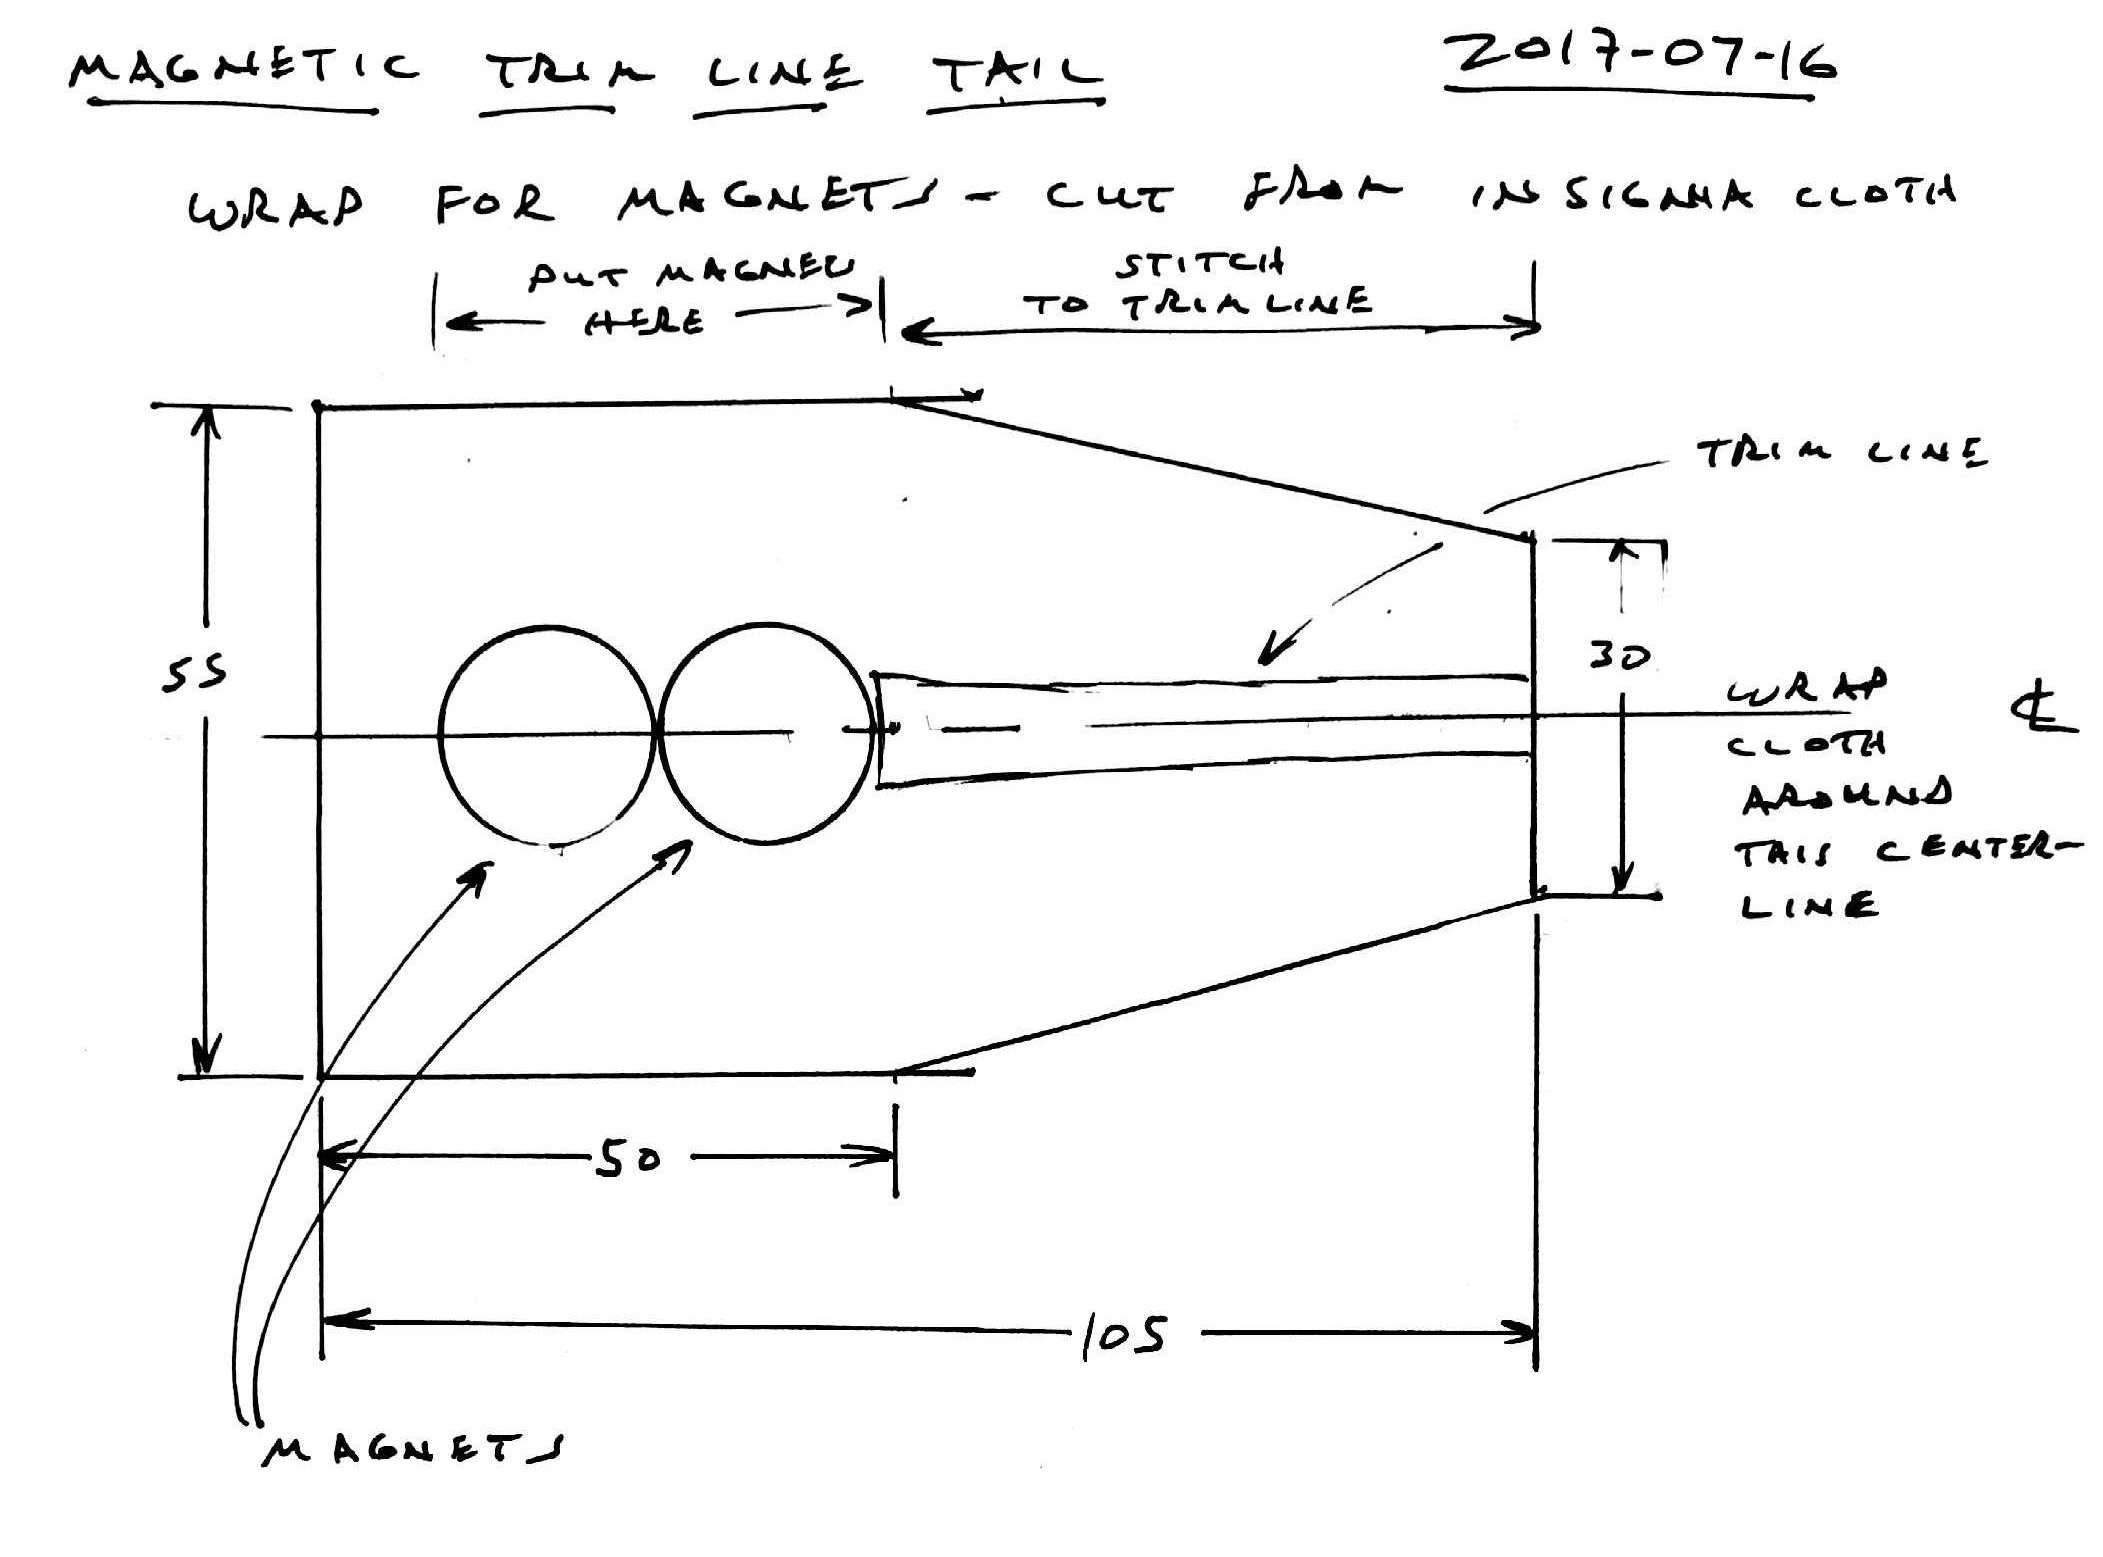
\includegraphics[width=0.7\linewidth]{images/magnetic_trimline_tails_9} 

}

\caption{Insignia cloth patch to hold trimline magnets}\label{fig:magnet-wrap}
\end{figure}

Cut a segment of round, 0.95" diameter weed-whacker cord 150mm long to wrap around the magnets and up the trip line. Heat the middle of the plastic cord with a low flame, bend it 180 degrees around the 18mm curve of one of the disc magnets and cool it under tap water. Dry the plastic and magnet so they are ready to be glued. Taper the last 15mm of the tips of the plastic cord so it can fit more closely against the trim line. The taper should be on the interior faces of the plastic cord.

Cut a strip of insignia cloth 20mm x 90mm to use as wrap and threading end on one end of the trim line.

Using the 4mm Amsteel as the foundation of the trimline, pick out 4 strands from one end of line pulling one strand at each of 5, 10, 15, and 20mm to form a tapered end. Cut each strand off with a razor blade. Wrap the last 30mm of that end of the trim line with the 20 x 90mm insignia cloth wrapping the 20mm dimension tightly around the Amsteel. 60mm of the cloth will extend past the end of the line. Fold this portion of the cloth on itself as you wrap to form a long, narrow, flat strip.

\begin{figure}

{\centering 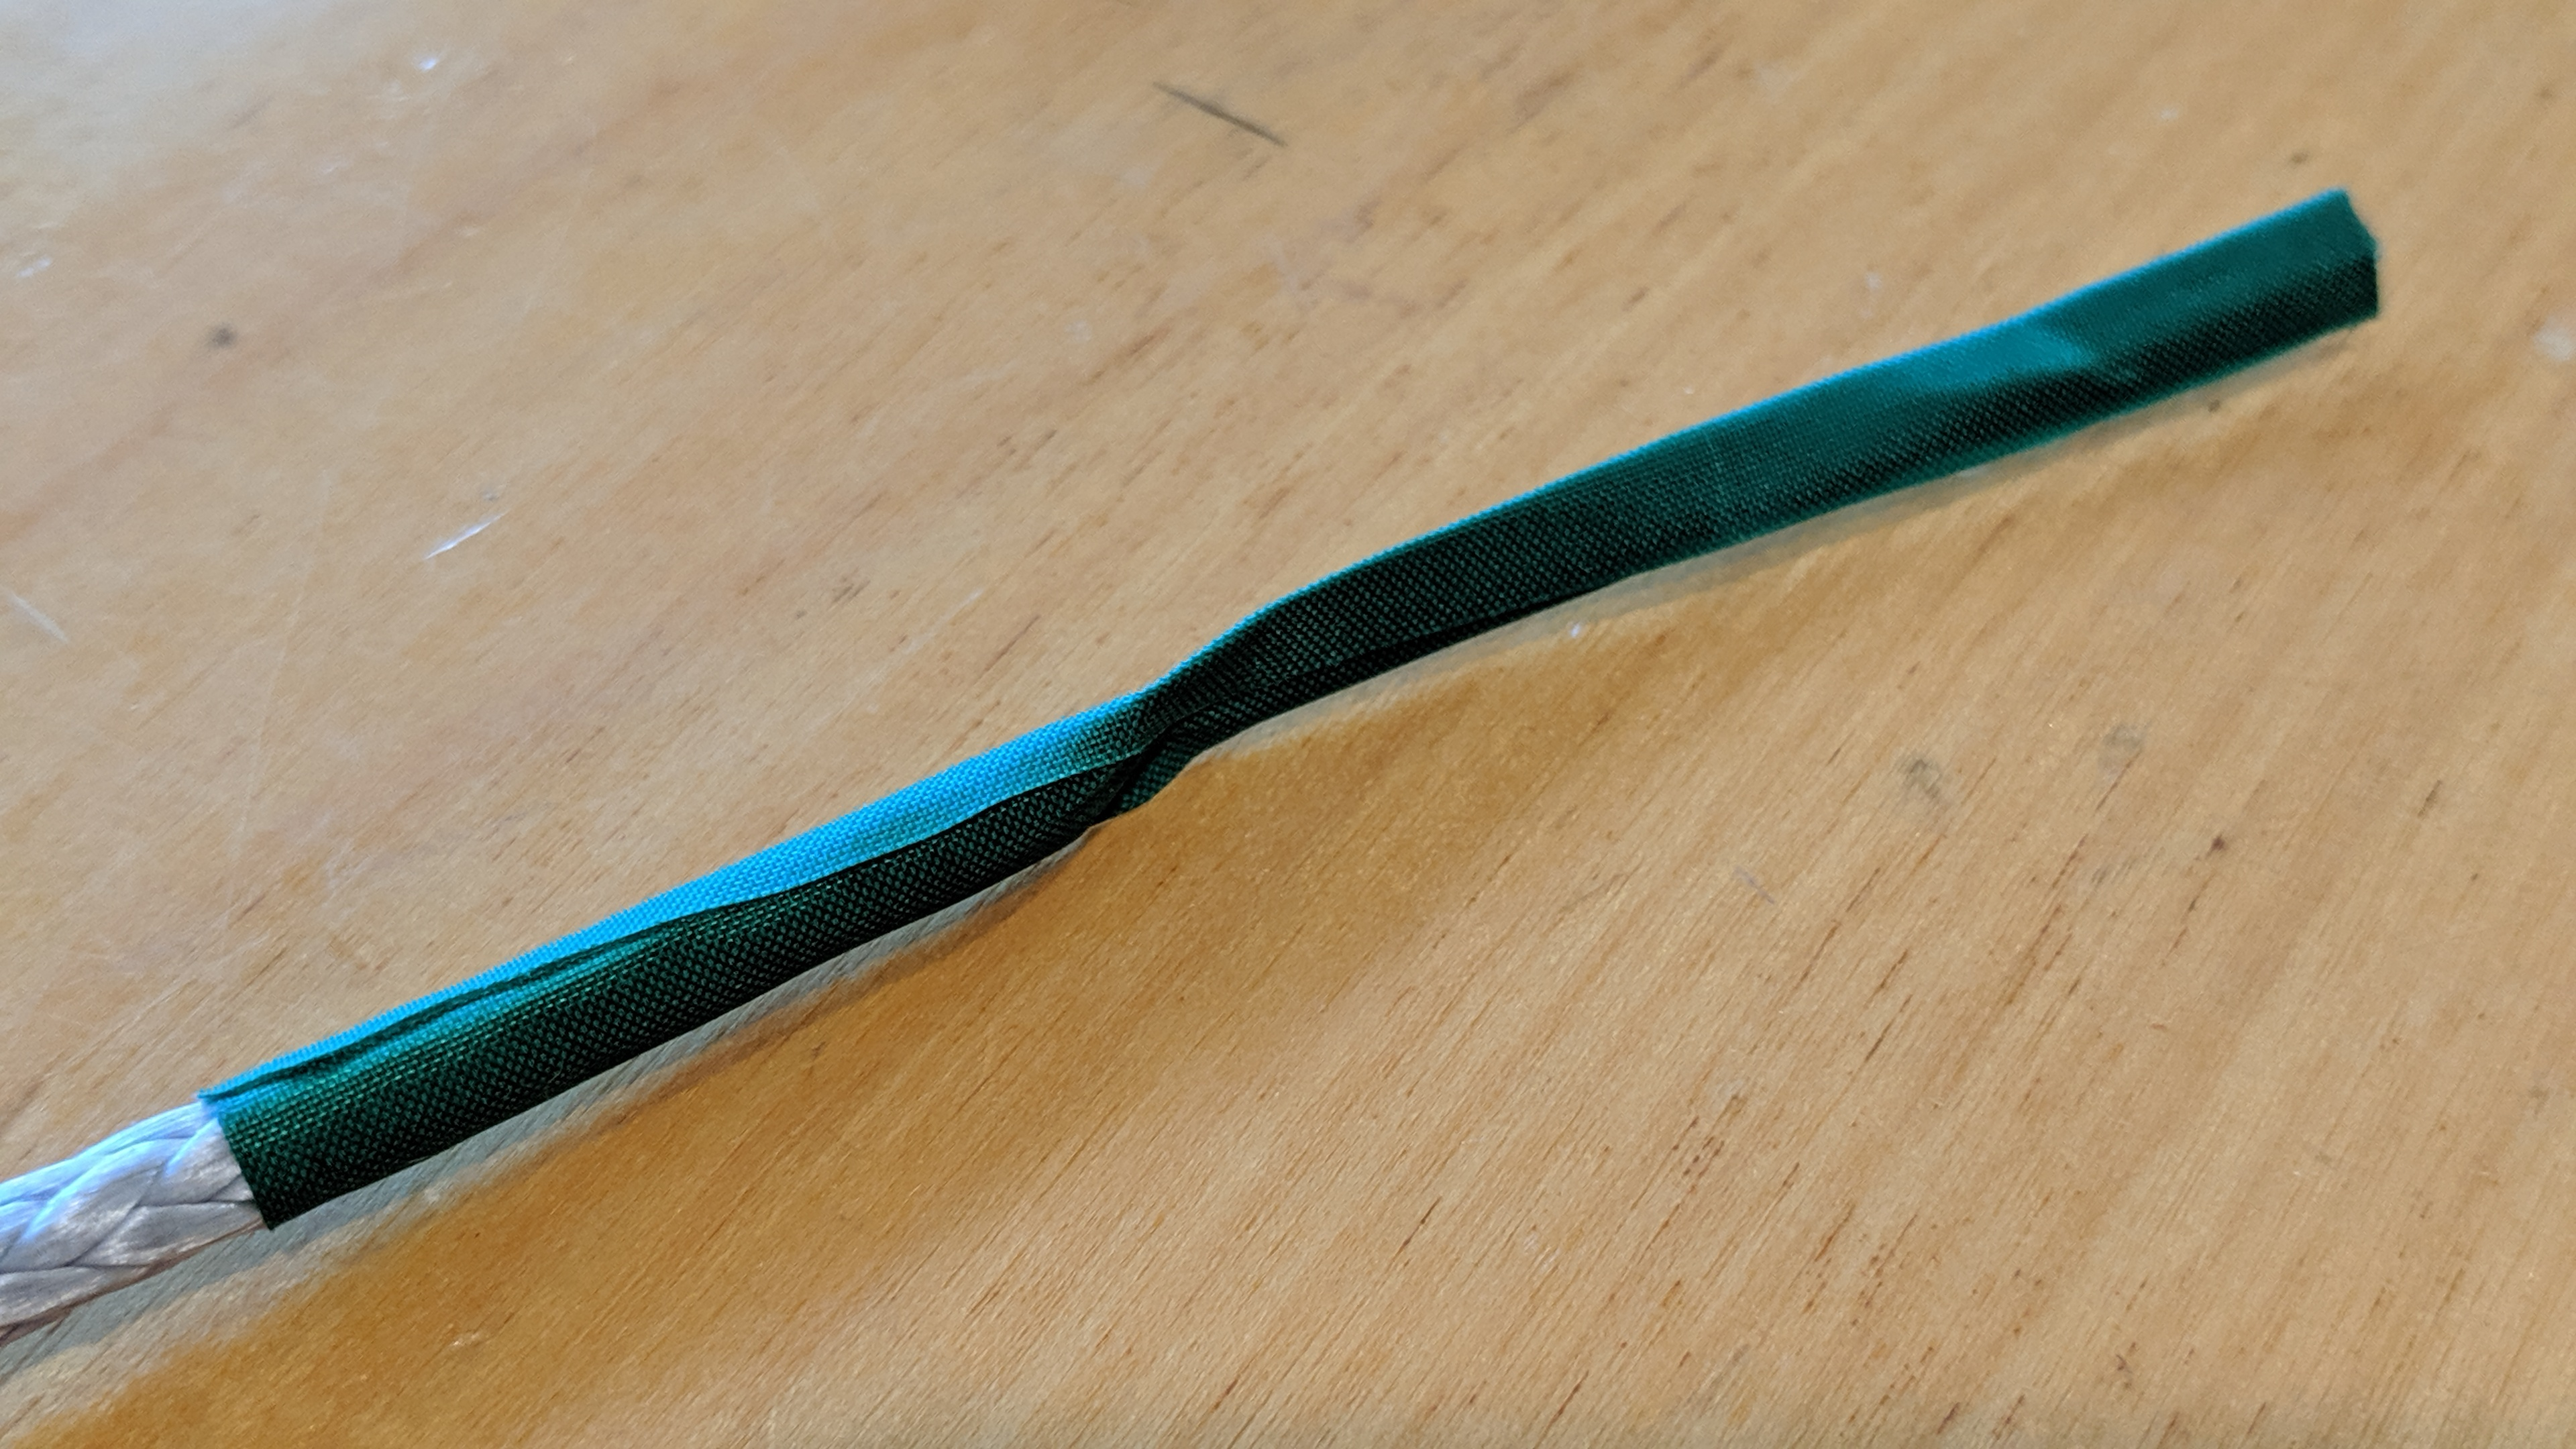
\includegraphics[width=0.7\linewidth]{images/thread_end_of_trimline} 

}

\caption{Threading end of the trim line formed with a wrap of insignia cloth}\label{fig:thread-end}
\end{figure}

To form the other end of the trimline, place 55mm of the unfinished end of the Amsteel on the tapered end of the magnet wrap. In your hand, place two 18mm x 3mm disc magnets edge-to-edge and align the polarity. Carefully place the pair of magnets edge-to-edge at the tip of the Amsteel aligning the long axis of the magnets with the axis of the Amsteel. The result should look like Figure \ref{fig:thread-end}.

Place the curve of the plastic cord closely around magnets. The tapered ends of the plastic cord should fit closely around the trim line.

Fold the cloth around magnets and trim line. The folds should be parallel to the trim line axis. The cloth must lay flat over the magnets. Because the trim line is narrower than the magnets, a crease will form where the magnets meet the trim line. This crease must not be \emph{on} the magnets. Make sure the crease is \emph{above} the magnets. Pinch the cloth closed below the magnets.

Stitch the magnet-wrap to the Amsteel so the cloth won't creep in use. Use a triple zig-zag stitch and dark thread to secure the warp. The attractive force of the magnets is so high, it can make the trim difficult to work in a sewing machine. To reduce this effect, cut two small rectangles of cardboard from a cereal box and place them under the magnets. The increased distance between the magnets and the steel of the sewing machine should make the forces manageable. Be careful to not hit the magnets or the plastic cord with the sewing needle lest bad things happen.

Tie an overhand knot at the point where the magnet wrap meets the Amsteel. The knot should be just barely above the plastic cord buried inside the magnet wrap.

Thread a 25mm ball onto the trimline, recessed side first. Slide it all the way to the knot next to the magnet wrap. Mark the trimline 65mm above the top of the green ball. Tie and overhand knot in the trimline just above that knot. Now thread a 12mm ball onto the trim line and slide it all the way to the knot. The finished product can be seen in Figure \ref{fig:finished-end}

\begin{figure}

{\centering 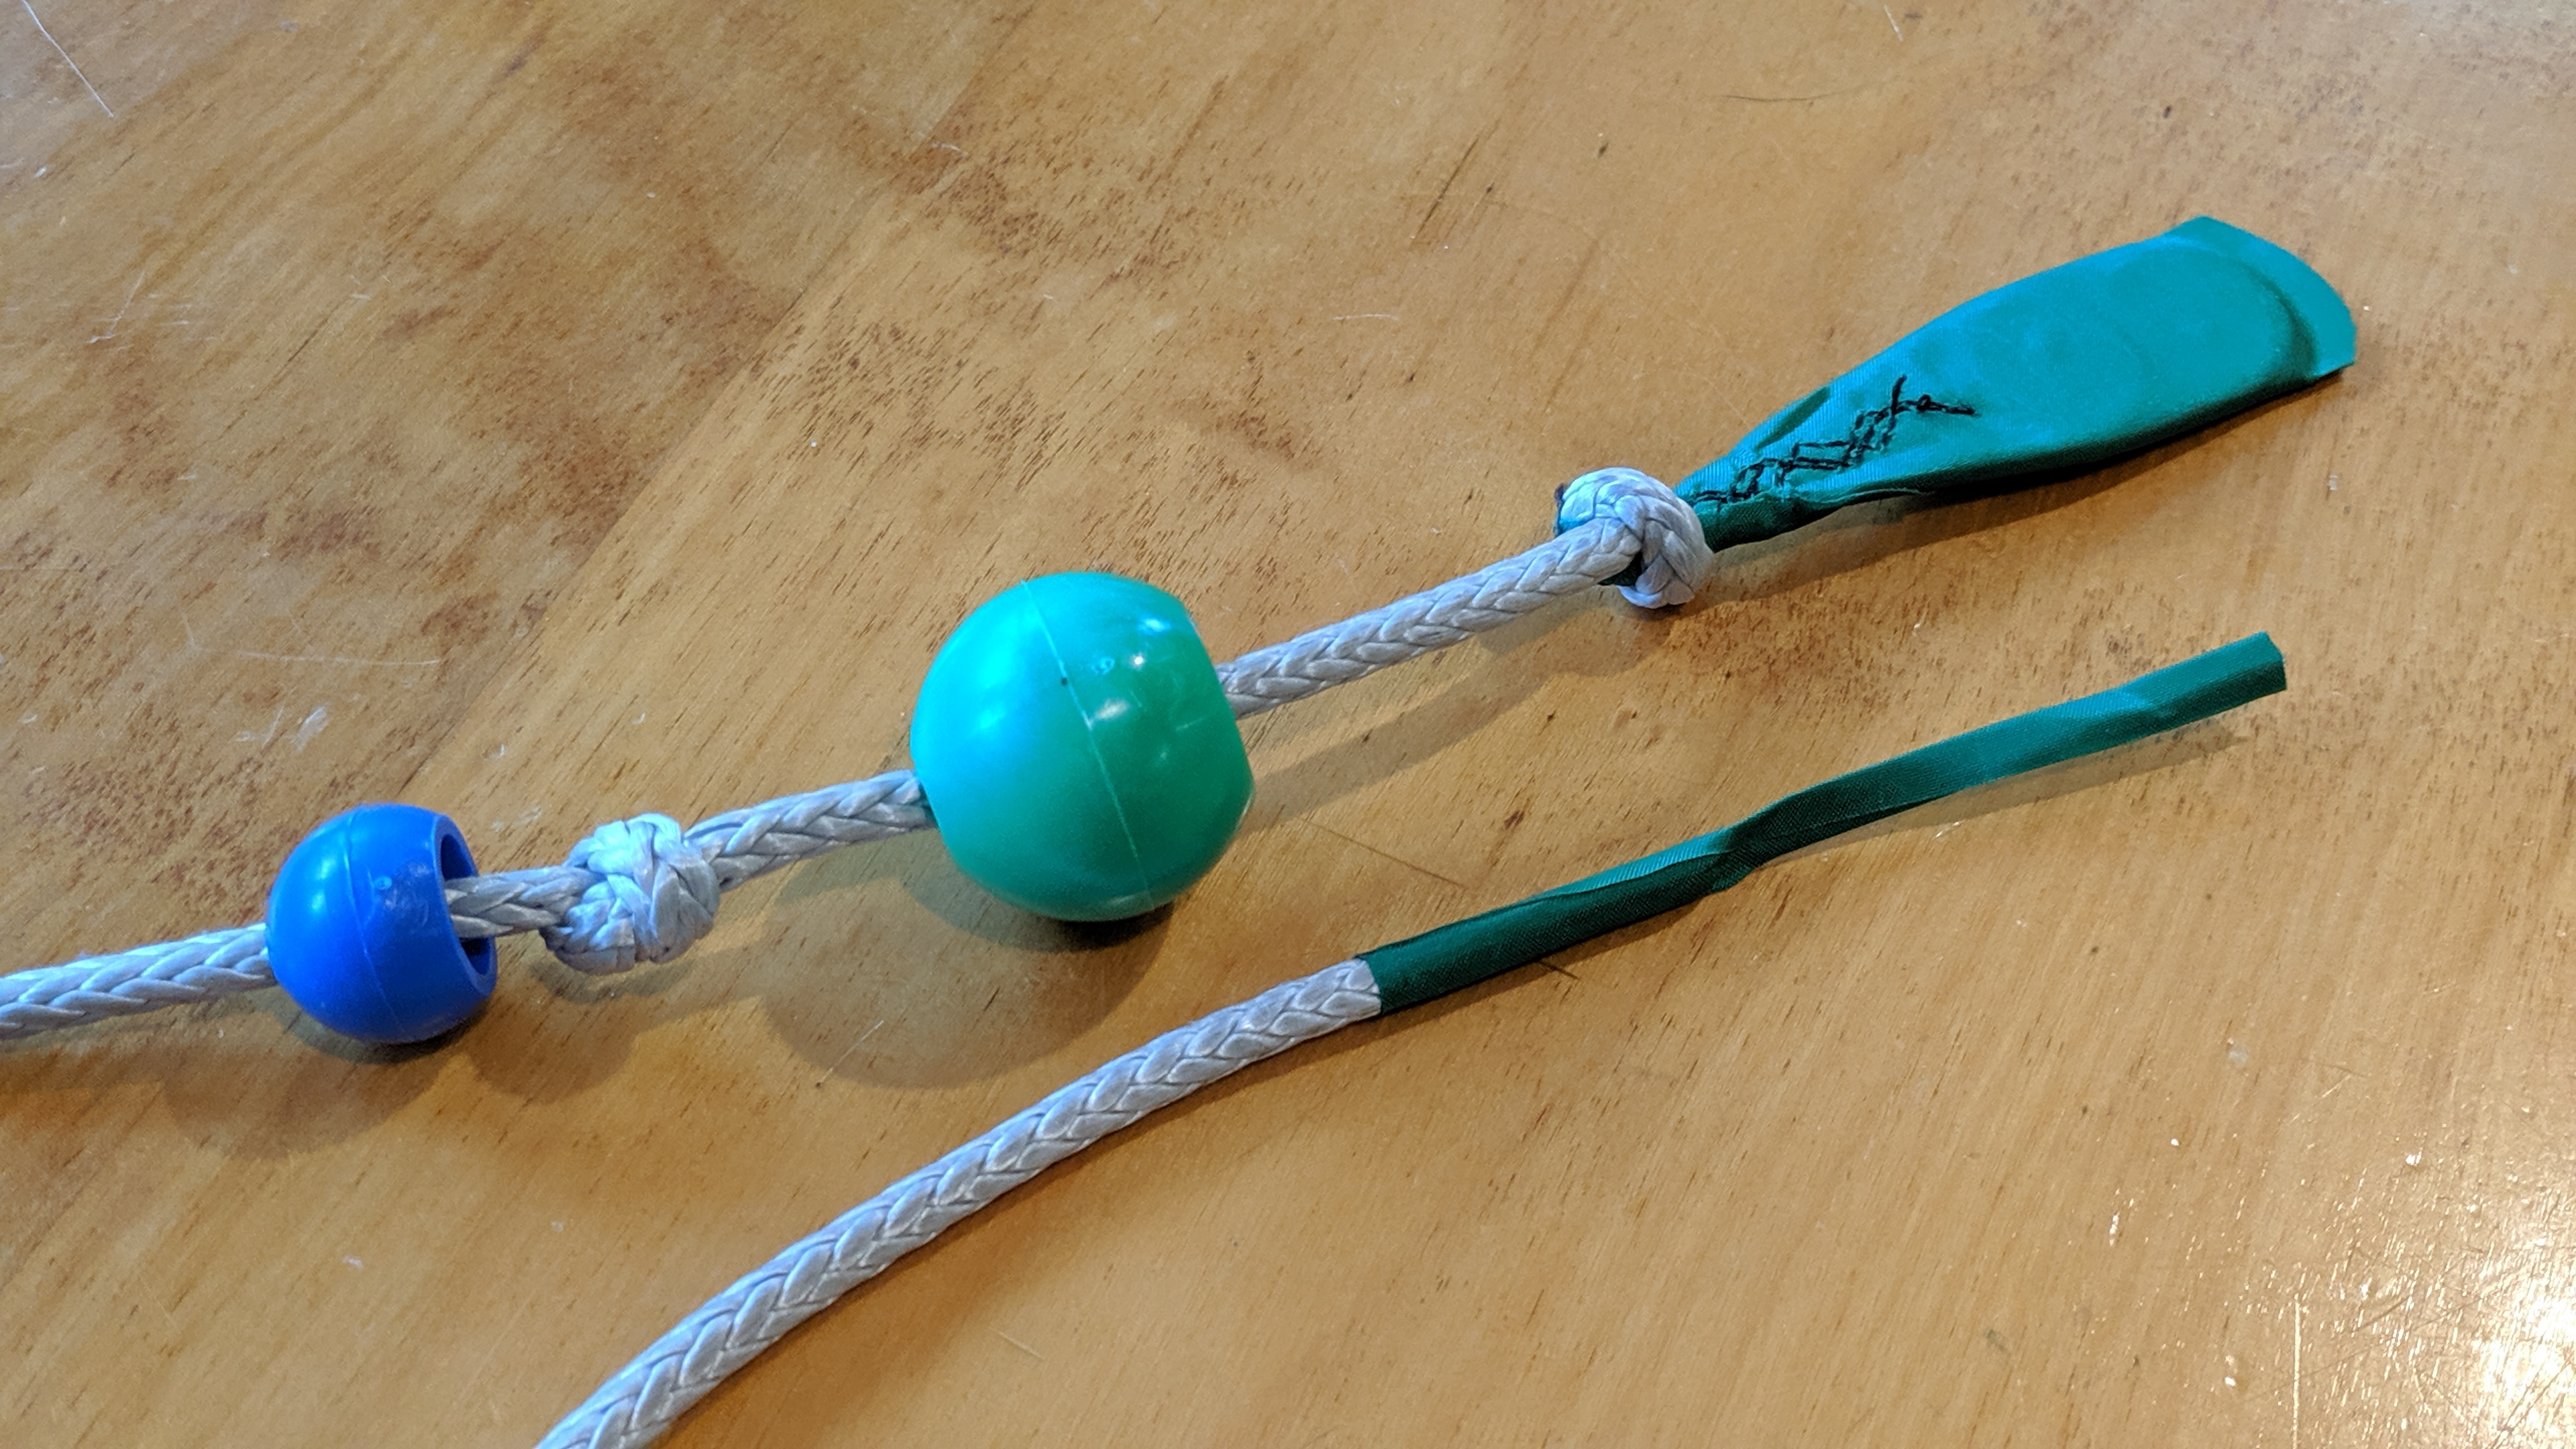
\includegraphics[width=0.7\linewidth]{images/finished_end_of_trimline} 

}

\caption{Grip end of the trim line with balls offset to show knots (above) and thread end (below)}\label{fig:finished-end}
\end{figure}

\hypertarget{cleat-jacket}{%
\section{Cleat Jacket}\label{cleat-jacket}}

The Aero Cleat requires a jacket of magnetic stainless steel sheet to create a tether point for the trimline tail. Make a template from the image in Figure \ref{fig:cleat-jacket-template}, trace the pattern onto a sheet of 0.025" thick 430 stainless steel sheet. You can also make your own template by placing the metal portion of the cleat into a piece of cardboard and tracing its outline on 3 sides or just trace it directly onto the metal. Cut the shape from the metal sheet, drill out the two holes with a 5/32" bit and ease all the edges with a metal file. Most of these edges will be on grippable surfaces, so do a good job of easing them.

Disassemble the cleat and reassemble it with metal sheet between the two sections of the cleat. Bend the metal sheet around the metal portion of the Aero Cleat. To do this, clamp one side of the jacket in a vise. Use a block of wood and a mallet to fold the other side against metal side of the cleat. Flip the cleat over to expose the unfolded wing of the jacket and clamp the cleat in the vise. Again, use the block of wood and a mallet to fold the remaining wing. Remove the cleat from the vise, lay it flat on a table top and use the block and mallet to crease the folds.

\begin{figure}

{\centering 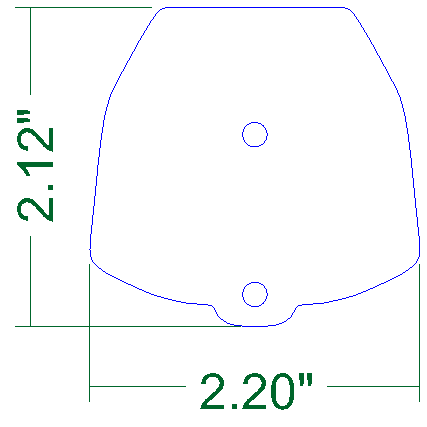
\includegraphics[width=1\linewidth]{images/cleat_jacket_template} 

}

\caption{Template for making an Aero Cleat Jacket}\label{fig:cleat-jacket-template}
\end{figure}

\hypertarget{separation-block-and-low-friction-ring}{%
\section{Separation block and low friction ring}\label{separation-block-and-low-friction-ring}}

The juncture of the flying lines and the trim line is managed by an assembly of a plastic block known as the separation block and a low friction ring connected via a spliced length of 7/64" Amsteel.

To build the assembly, you will need 295mm of 7/64" Amsteel Blue (preferably gray), two 20mm x 65mm rectangles of insignia cloth, one FR5 Tylaska Rigging Ring Ferrule or similar, and one Separation Block release 1.4.2.

Pick out 4 strands from one end of Amsteel pulling out one strand at each of 5, 10, 15, and 20mm to form a tapered end. Cut each strand off with a razor blade. Wrap that end of theAmsteel with a rectangle of insignia cloth. Wrap the 20mm dimension around the line with 30mm on the line and 35mm off. The result should look Figure \ref{fig:unfinished-separation-block-cord}

\begin{figure}

{\centering 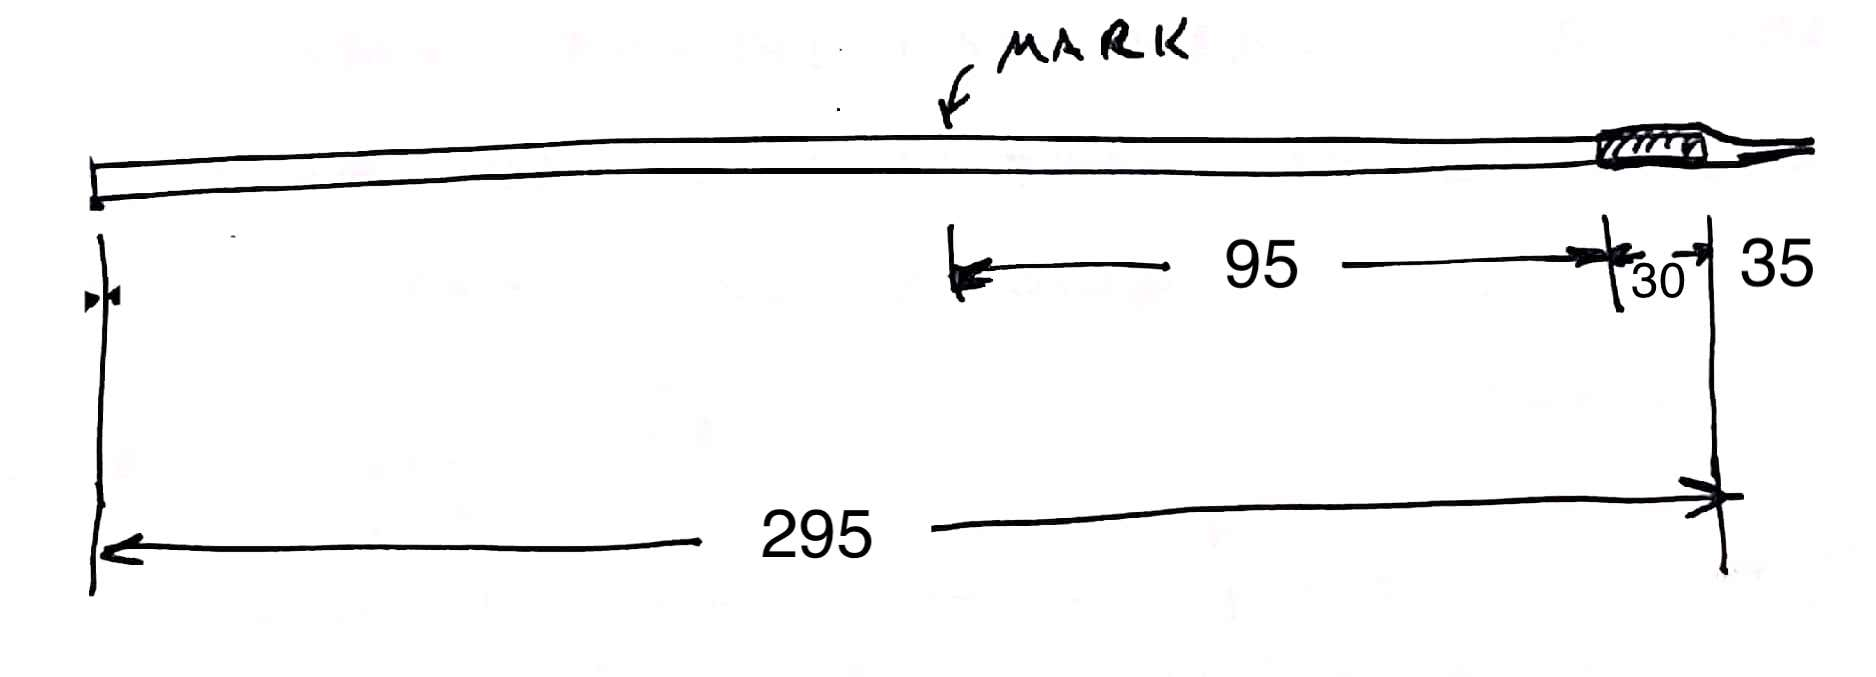
\includegraphics[width=0.7\linewidth]{images/unfinished_separation_block_cord} 

}

\caption{Unfinished separation block cord}\label{fig:unfinished-separation-block-cord}
\end{figure}

Measure 95mm from the tip of the tapered line. Pierce the line at 95mm and start a brummel splice at the mark. Place the low-friction ring inside the loop. Pull the loop tight around the ring. Run a wire fid from a point 20mm from the opposite end of the line. Pop the fid out of the line at the ring. Use the wire fid to pull the tapered end inside. When you pull the end of the tapered end out, peel off the extra insignia cloth before you bury it. Use the second piece of insignia cloth to put a threading end on the finished piece. The result should have the dimension in Figure \ref{fig:finished-separation-block-cord}. It should look like the picture in Figure \ref{fig:finished-separation-block-cord-pic}

\begin{figure}

{\centering 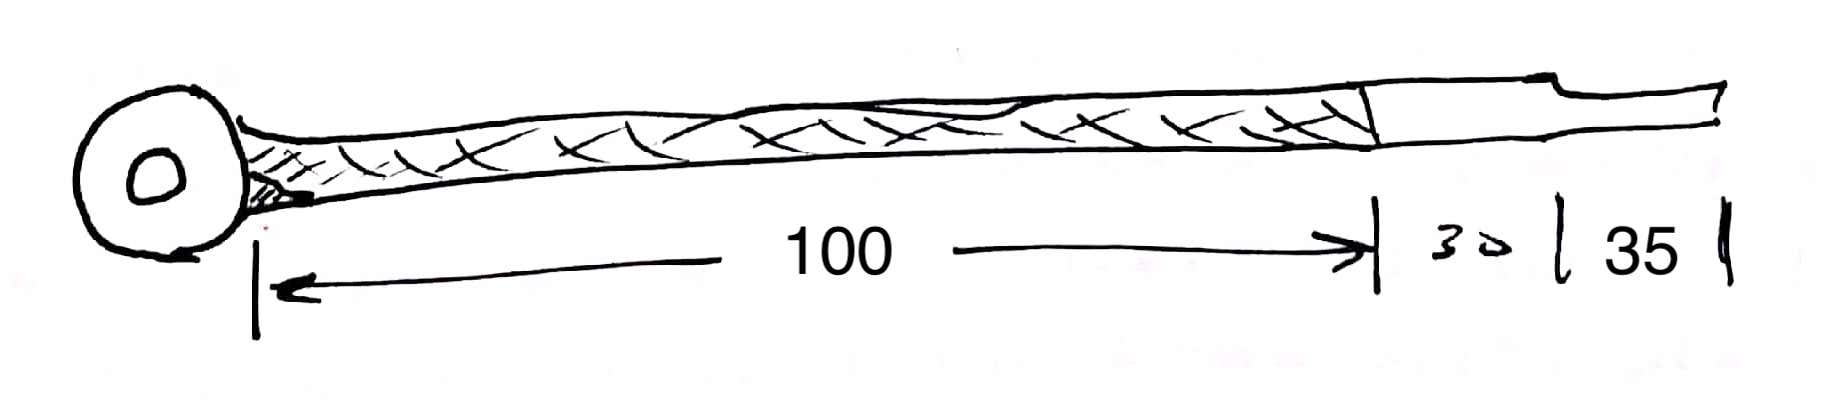
\includegraphics[width=0.7\linewidth]{images/finished_separation_block_cord} 

}

\caption{finished separation block cord}\label{fig:finished-separation-block-cord}
\end{figure}

\begin{figure}

{\centering 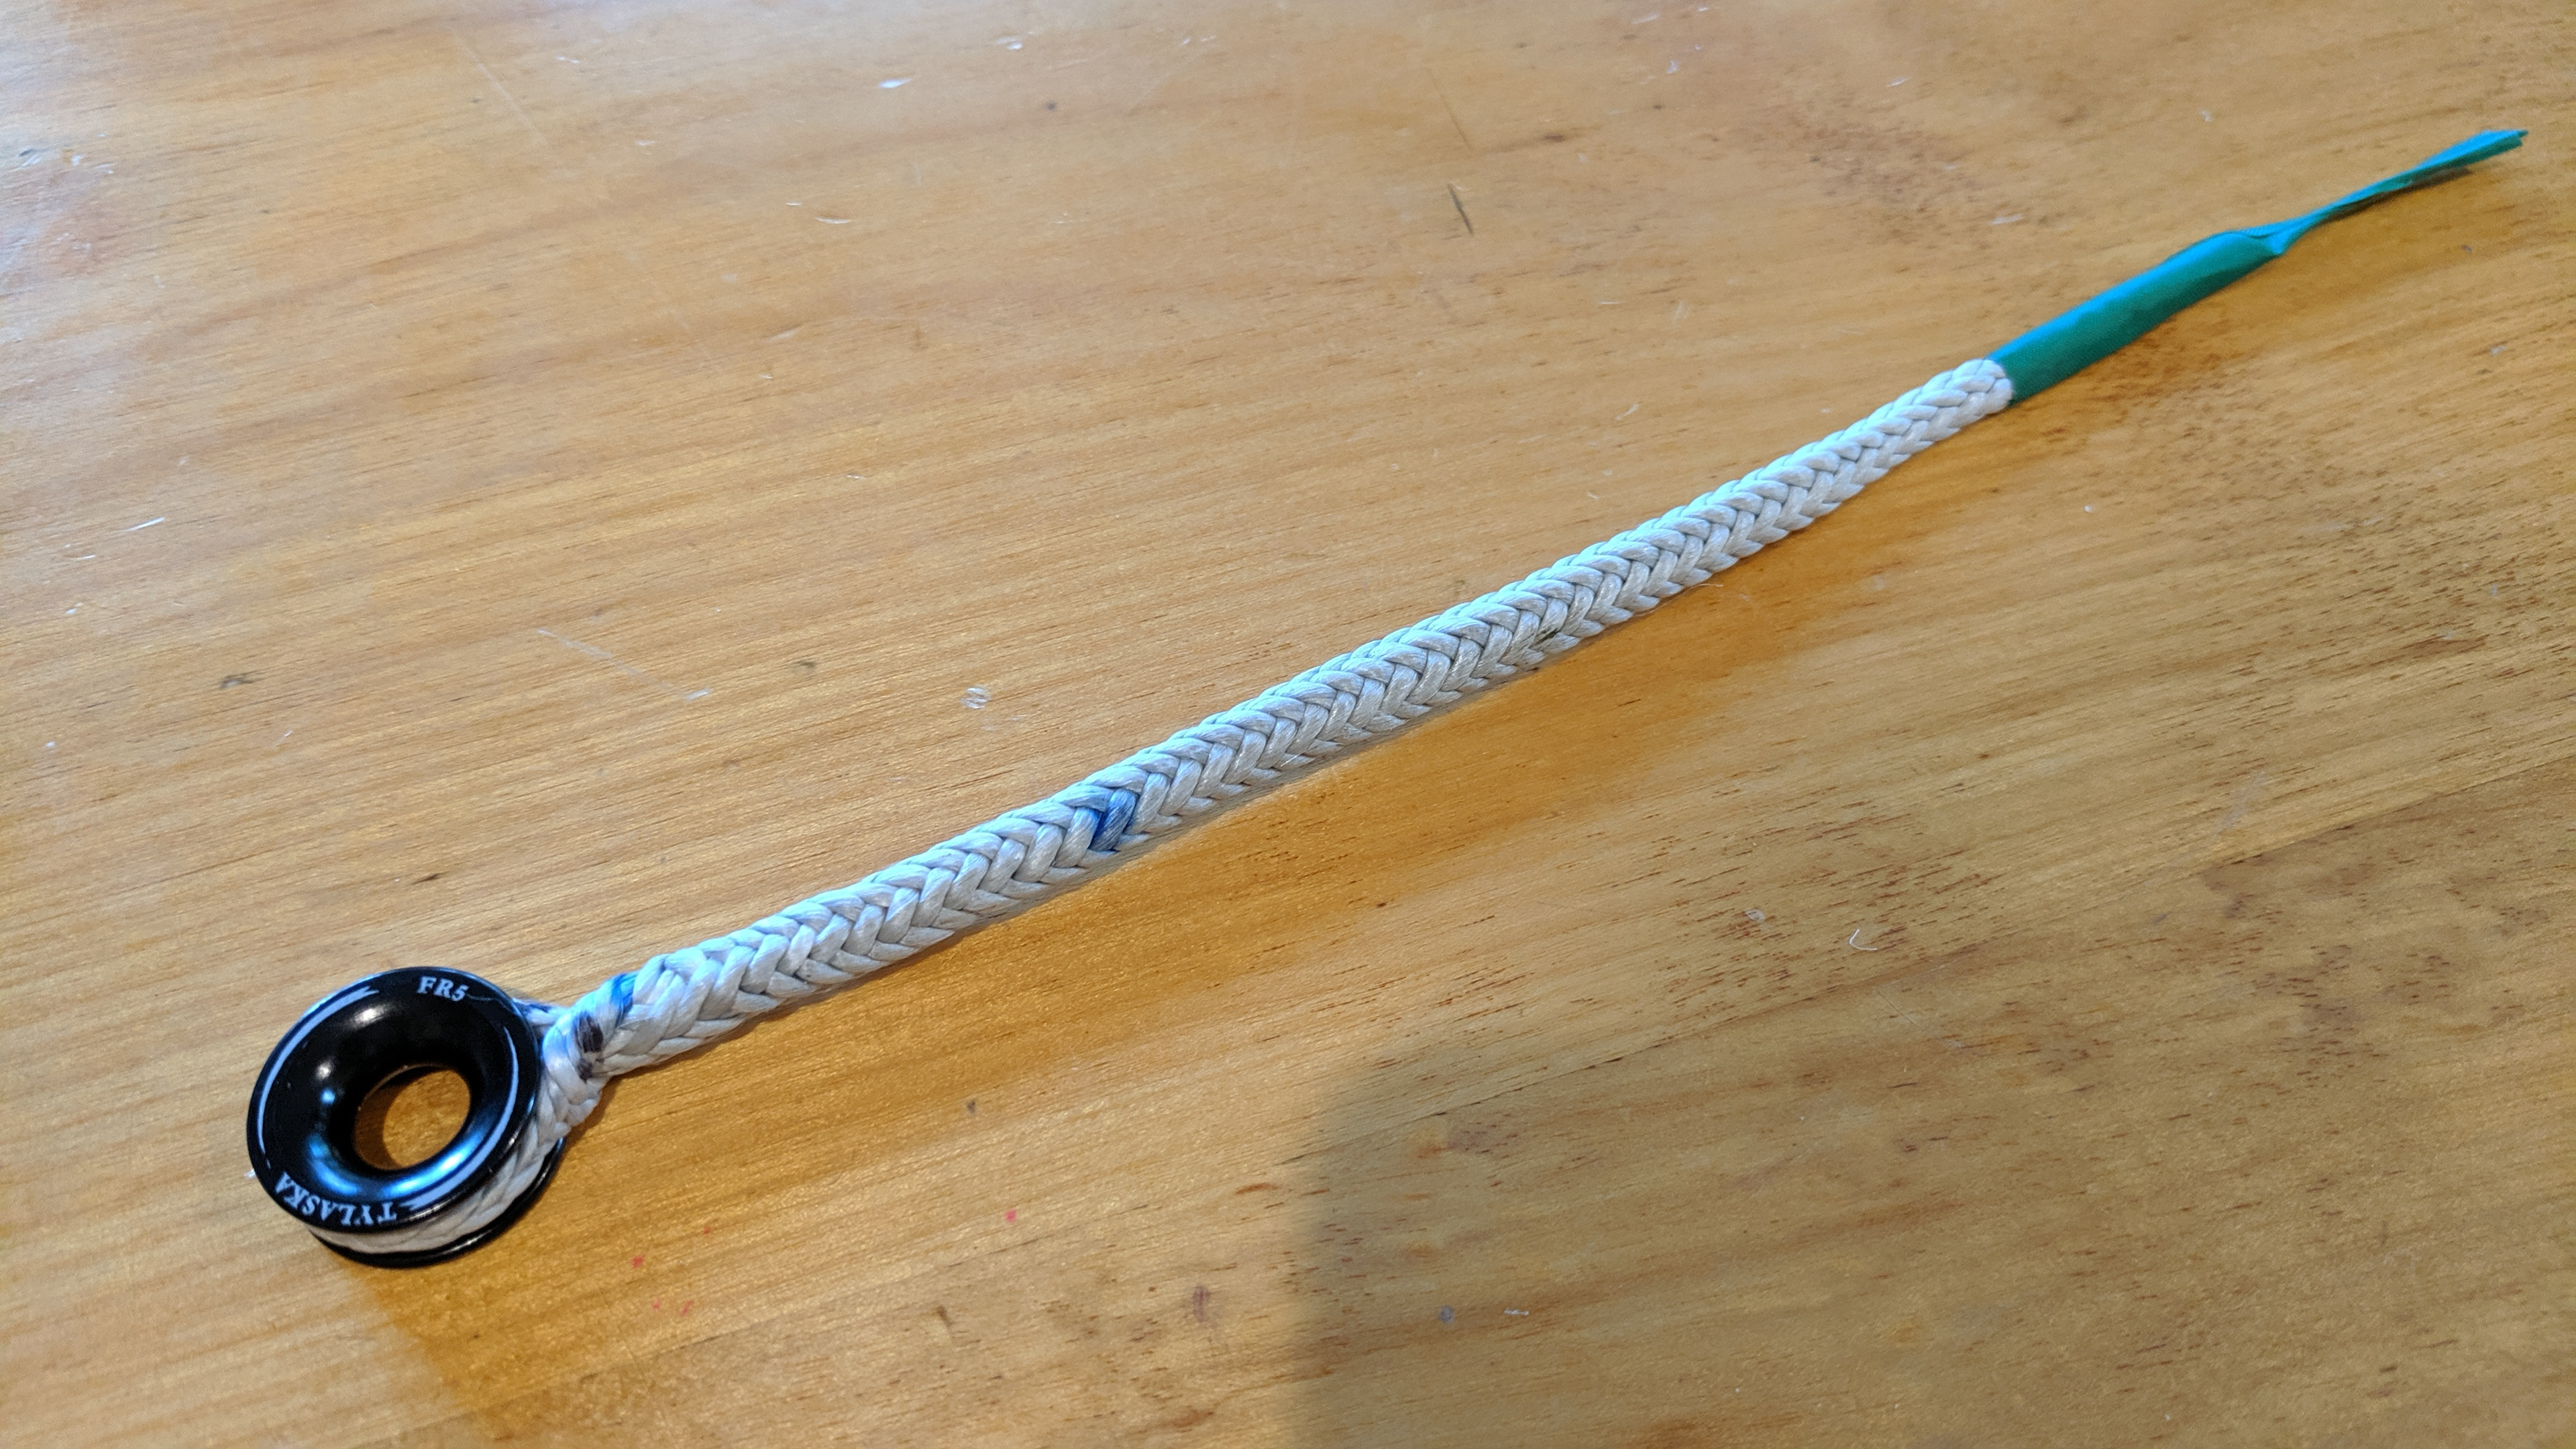
\includegraphics[width=0.7\linewidth]{images/finished_separation_block_cord_pic} 

}

\caption{Picture of a finished separation block cord}\label{fig:finished-separation-block-cord-pic}
\end{figure}

Thread the resulting line-ring assembly through the center bore of the separation block. Tie an overhand knot in the Amsteel taking out as much slack as possible. The completed assembly is show in Figure \ref{fig:finished-separation-block-assembly}

\begin{figure}

{\centering 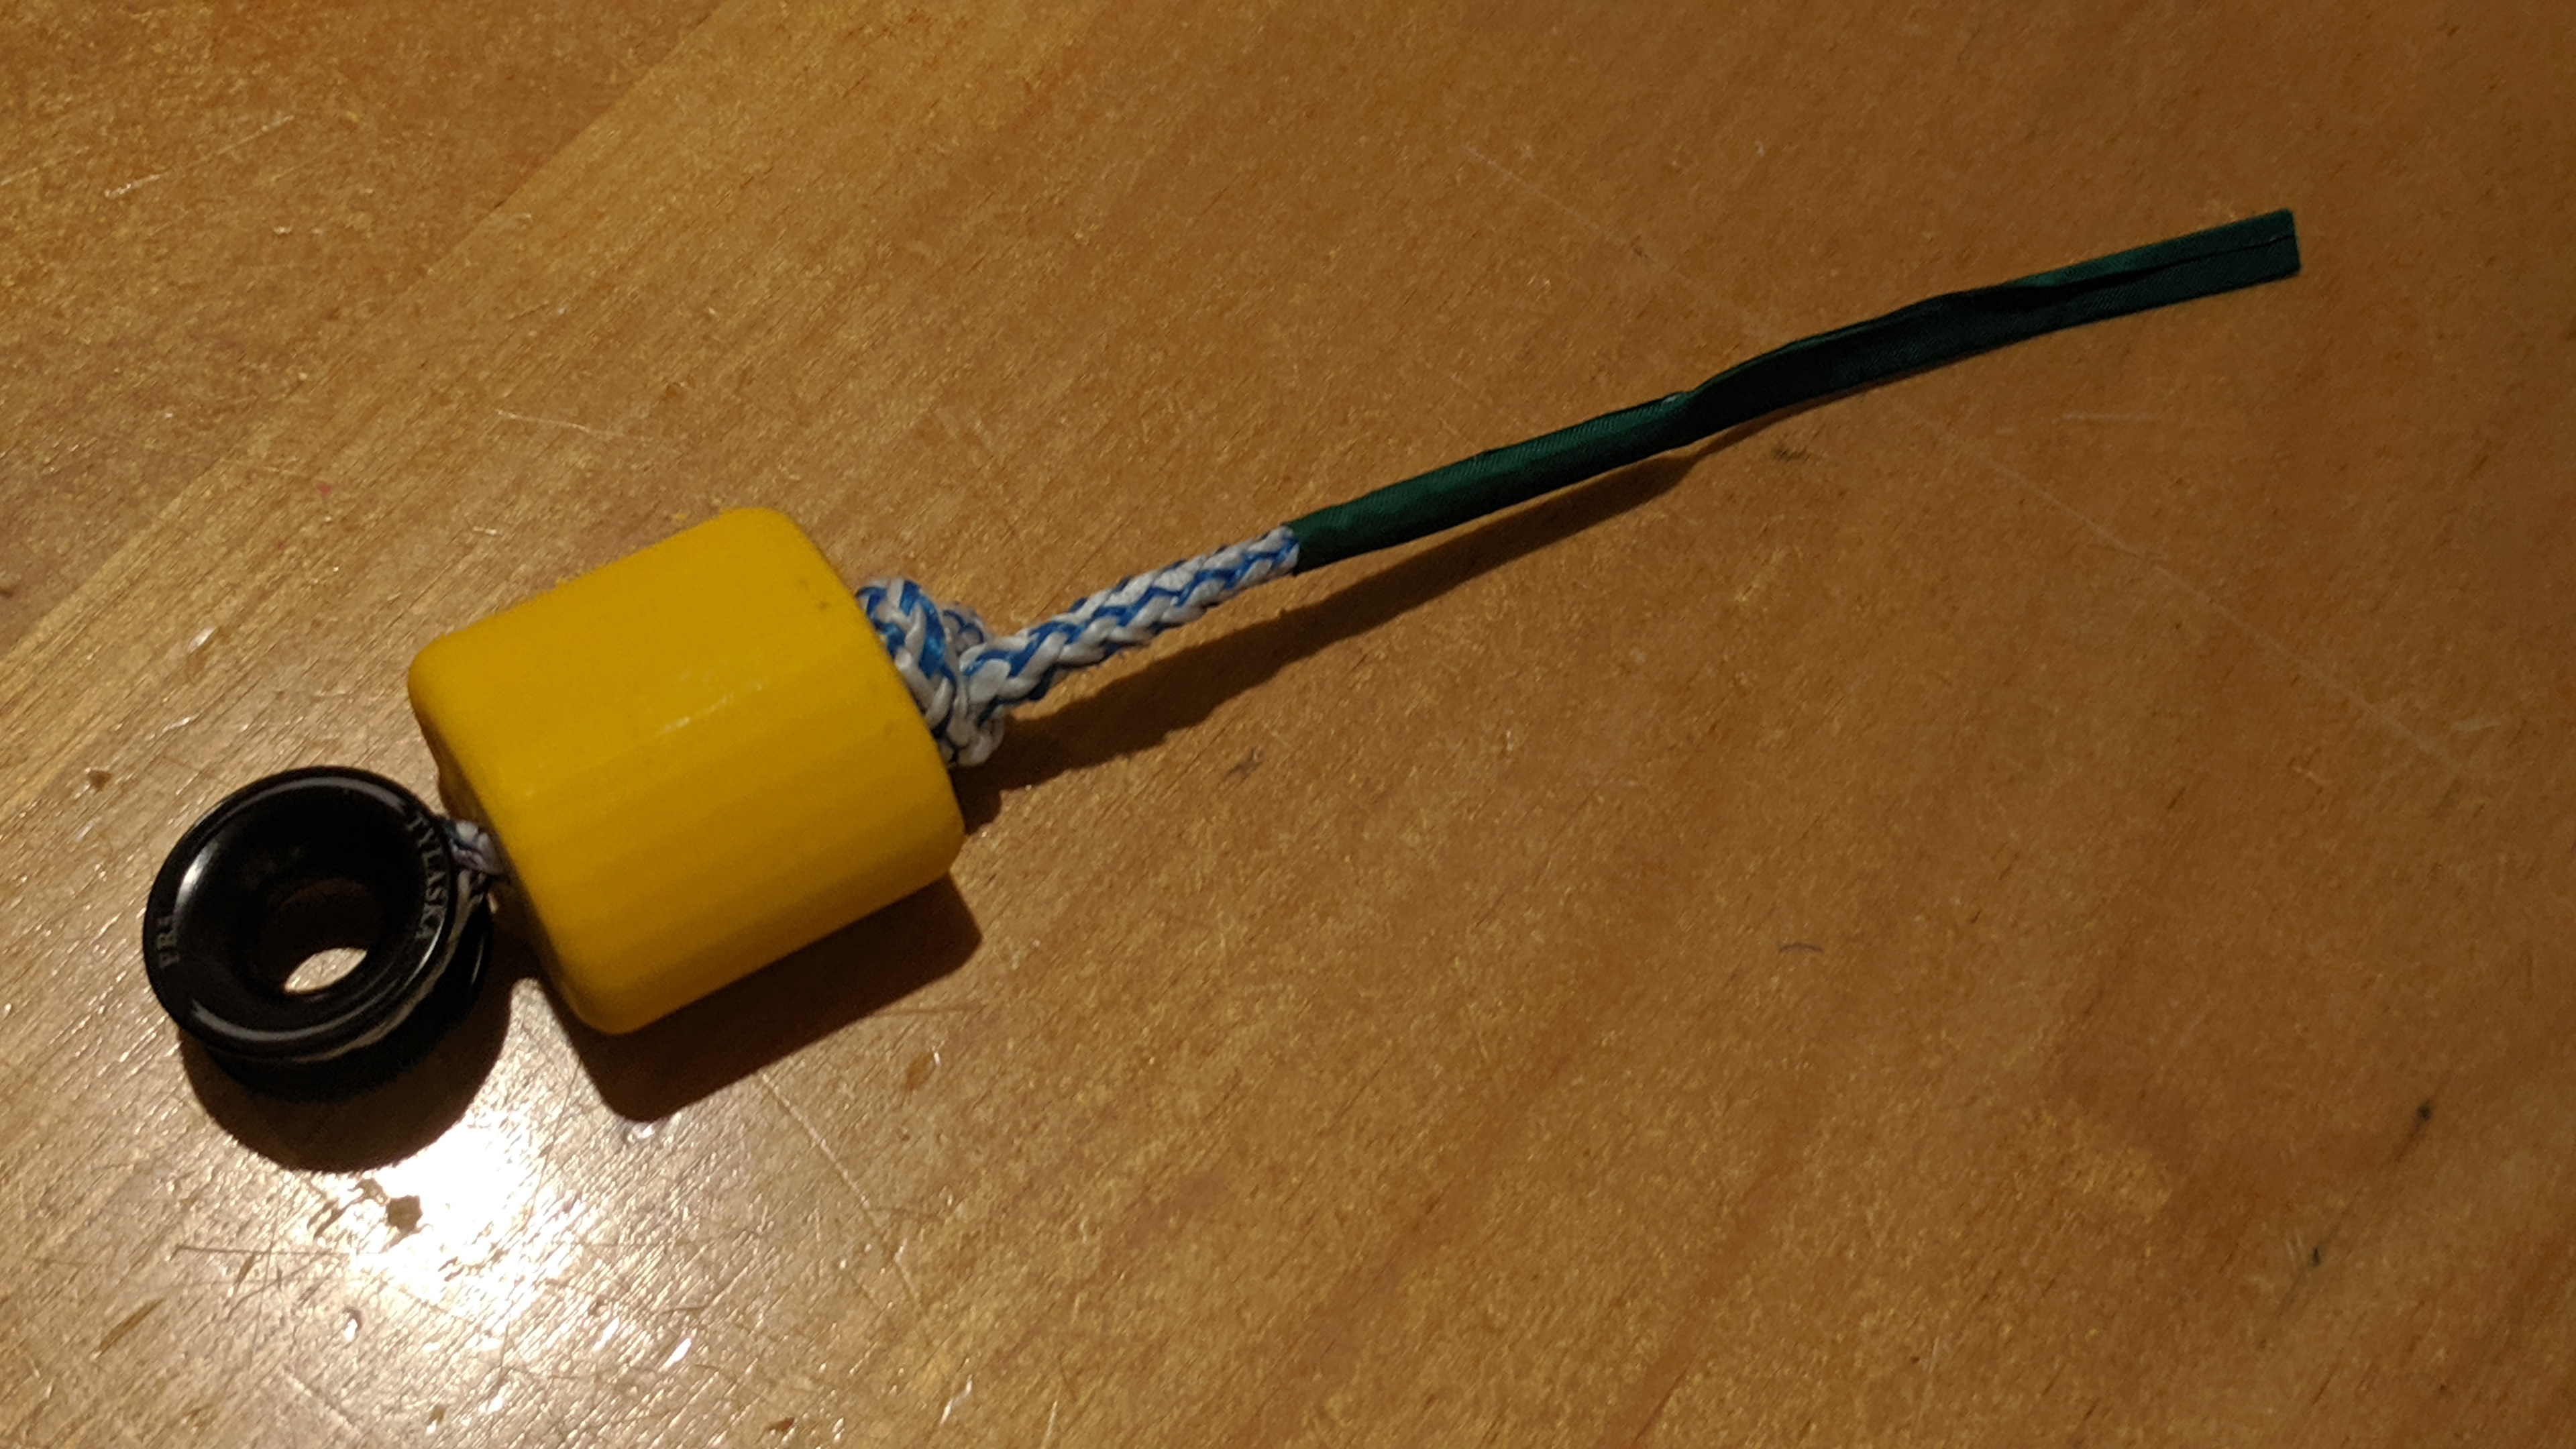
\includegraphics[width=0.7\linewidth]{images/finished_separation_block_assembly} 

}

\caption{Picture of separation block assembly}\label{fig:finished-separation-block-assembly}
\end{figure}

\hypertarget{flag-line}{%
\section{Flag line}\label{flag-line}}

The \emph{flag line} allows the kite to be flagged out via one of the top lines. It bridges the distance from the flying line at the underside of the separation block and the underside of the kite bar. The line is about 1400 of 1/16" Ultrex 12 that jackets about 400mm of 2mm bungie. A short loop is incorporated into each end. This design allows the flag line to stay taught whether the bar is trimmed in or out. The Ultrex jacket can handle the loads experienced during release to assure a clean flag-out without damage to flag line. The dimensions for the flag line are tightly constrained by the need to maintain line tension throughout the trim range. They can be calculated using a copy of the Google Sheet \href{http://tinyurl.com/y4k5chgv}{kite bar elastic flag line length calculations} (\url{http://tinyurl.com/y4k5chgv})

To build the flag line, cut 1370mm of 1/16" Ultrex 12. Mark each end at 45mm, 65mm, 85mm, and 140mm. The 65mm will be the end of the loop while the 45mm and 85mm marks will align at the bottom of the loop. Make a brummel splice at one end to secure that loop. At other end, form the first loop of the brummel splice before splicing a line segment of about 40mm into the flag line between the 45mm and 85mm marks. Complete the brummel splice, and cut the ends off the short added segment and bury the remainder.

Unspool a meter of 2mm bungie and add a threading end of insignia cloth to the free end (use a 8mm x 40mm rectangle of cloth) . Measure 390mm from the back-end of the thread end and mark this point with a strip of insignia cloth. Route a very long fid inside the flag line from the near end of one loop to the near end of the other. The fid should occupy the entire length of the otherwise unoccupied flag line. Pull the 2mm bungie through the jacket and out the opposite end until only the thread end cloth is visible. Clamp this end with a spring clip. Align the strip of insignia cloth with the other entry-point into the flag line jacket. Clamp this end with the other spring clip.

Put the flag line under tension and start milking the jacket back and forth to evenly distribute the jacket and bungie. Use a 2m long stick and some cord to place the flag line under continuous tension. Continuing milking the jacket back and forth until it stops elongating. Retension the flag line and milk it again. With the flag line still stretched and the bungie still constrained by spring clips, sew the length of the flag line from spliced loop to spliced loop, back stitching at each end and on the ends of the bungie. Use a straight stitch.

Remove the spring clips and cut off the bungie that protrudes from the jacket. The bungie must be fully hidden inside the jacket to assure smooth operation.

To the lower end of the flag--the end that has not been fattened--affix a quick-release tether. The tether will require one 2" cotter pin, 40mm of 1/2" OD vinyl tubing, 200mm of 1/16" Ultrex 12, \textasciitilde{}100mm of 2mm bungee, and the end of the handle from a plastic bucket.

Cut the end off the bucket handle and round it to form two parallel disks connected at their centers. You are creating the yellow object in the picture below. Cross drill through the vinyl tubing about 5mm from the end with a 1/16" bit. Cut the cotter pin down to 40mm and round the end on coarse stone. splice the 200mm of Ultrex to form a line with a loop on each end. One these line will need to accept the bucket handle end, so size it appropriately.

Larkshead the cotter pin and Ultrex line to the end of the flag line. Thread the 2mm bungie through the holes in the vinyl and the larkshead. Tie off each end of the bungie with an overhand knot to retain it. Leave a 5mm tail on each end. Tie off the second side of the bungie, cut it and apply cyanoacrylate glue to prevent fraying. Pull the Ultrex line down through the vinyl and slide the bucket handle end into the the loop. A finished assembly--albeit with PVC in place of the vinyl--is shown in \ref{fig:flagline-disconnect}

\begin{figure}

{\centering 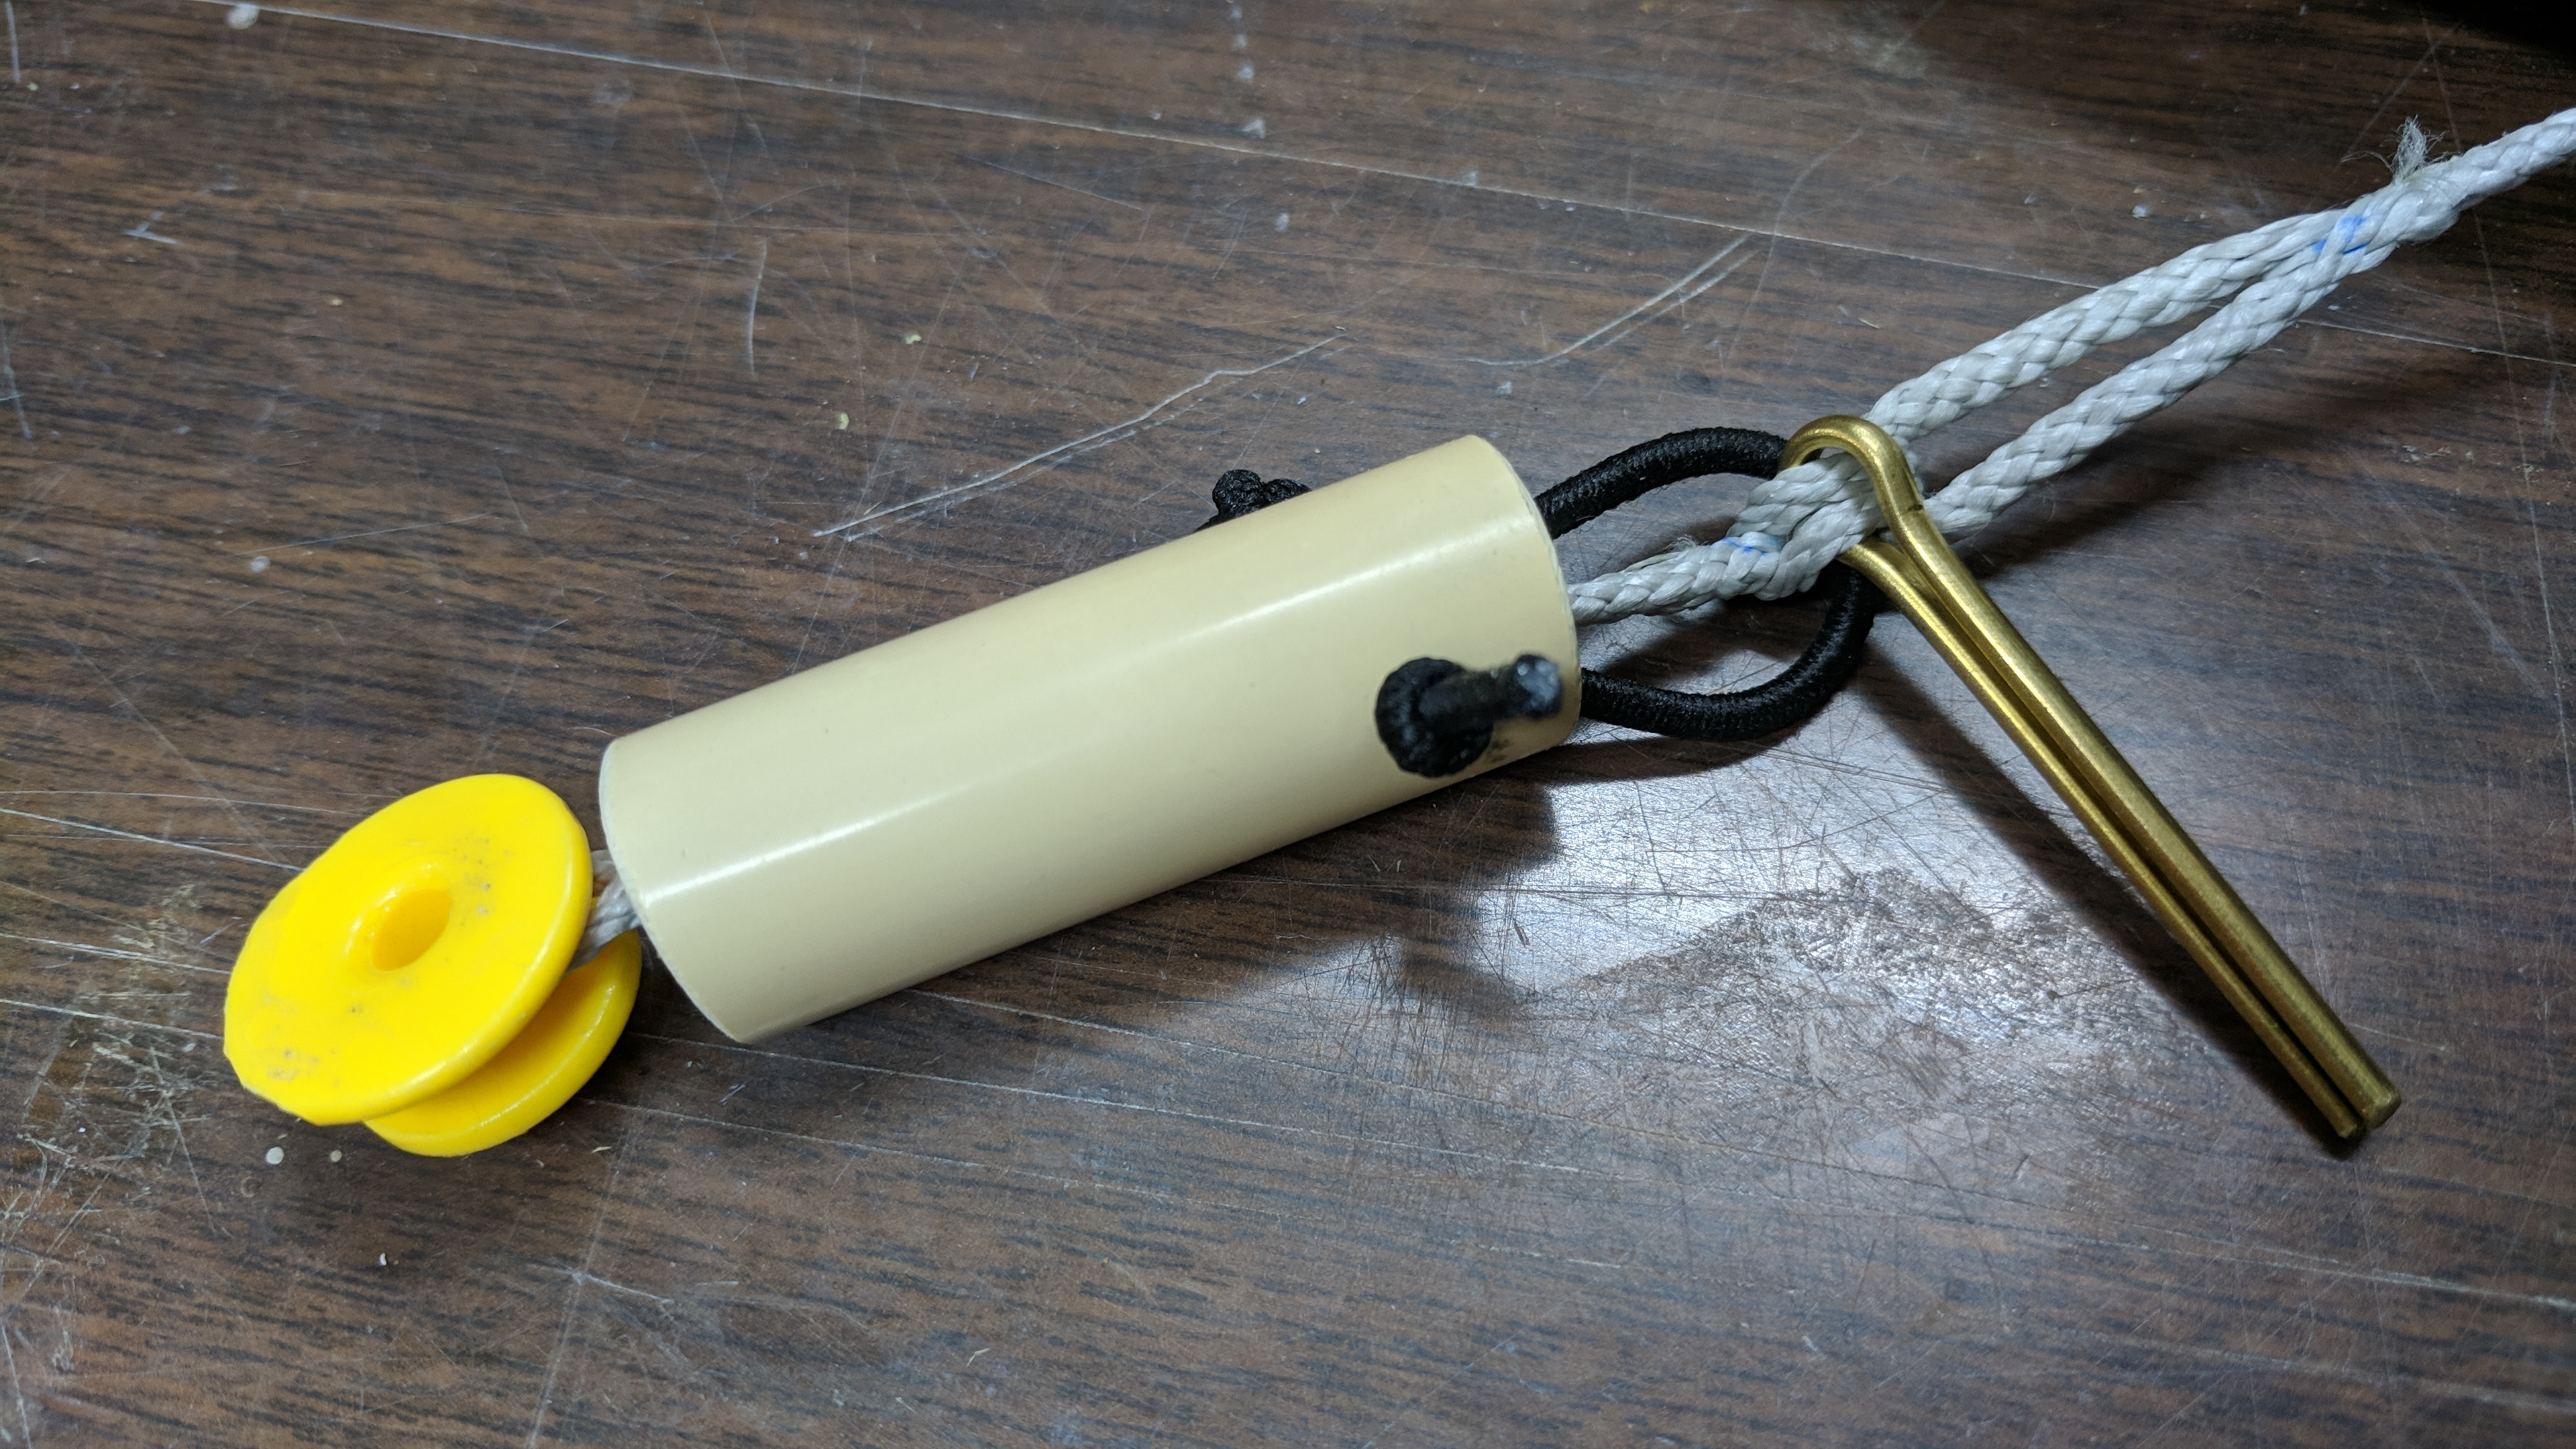
\includegraphics[width=0.7\linewidth]{images/flagline_disconnect} 

}

\caption{Flagline disconnect}\label{fig:flagline-disconnect}
\end{figure}

\hypertarget{stub-line}{%
\section{Stub line}\label{stub-line}}

The non-flagging flying line needs to be terminated at the underside of the separation block in the same manner as the flying line that \emph{does} flag. This is accomplished with a short loop called the \emph{stub line}. To match the upper end of the flag line, the stub line is made from 300mm of 1/16" Ultrex 12.

Mark the 300mm line segment 130mm from one end. Use a wire fid to splice the 130mm segment inside the 170mm segment that remains. The resulting segment will be about 155mm long. The segment is mostly double thickness with about 30mm of single thickness line on the end. Apply cyanoacrylate glue to the unfinished end. Fold the 155mm segment in half and tie an overhand knot to form a small loop. The finished product is about 50mm long.

\hypertarget{bar-end-loops}{%
\section{Bar End Loops}\label{bar-end-loops}}

The kite bar requires a loop on each end to affix the steering lines. These loops require two 350mm segments of 1/16" Ultrex 12. To make them fold each loop in half and tie an over hand knot at the end with about 10mm of tail. The length of these two lines \emph{must} match. To acheive this, hook the loop ends around a rounded component on a bench vise. Gently pinch the line with an adjustable wrench on the loop side of the knots. Use the wrench to pull the knots evenly while you pull the ends with standard pliers. With the knot complete and the lines equal in length, put little cyanoacrylate glue on the line ends to prevent fraying. See the detail diagram in Figure \ref{fig:bar-end-loop}.

\begin{figure}

{\centering 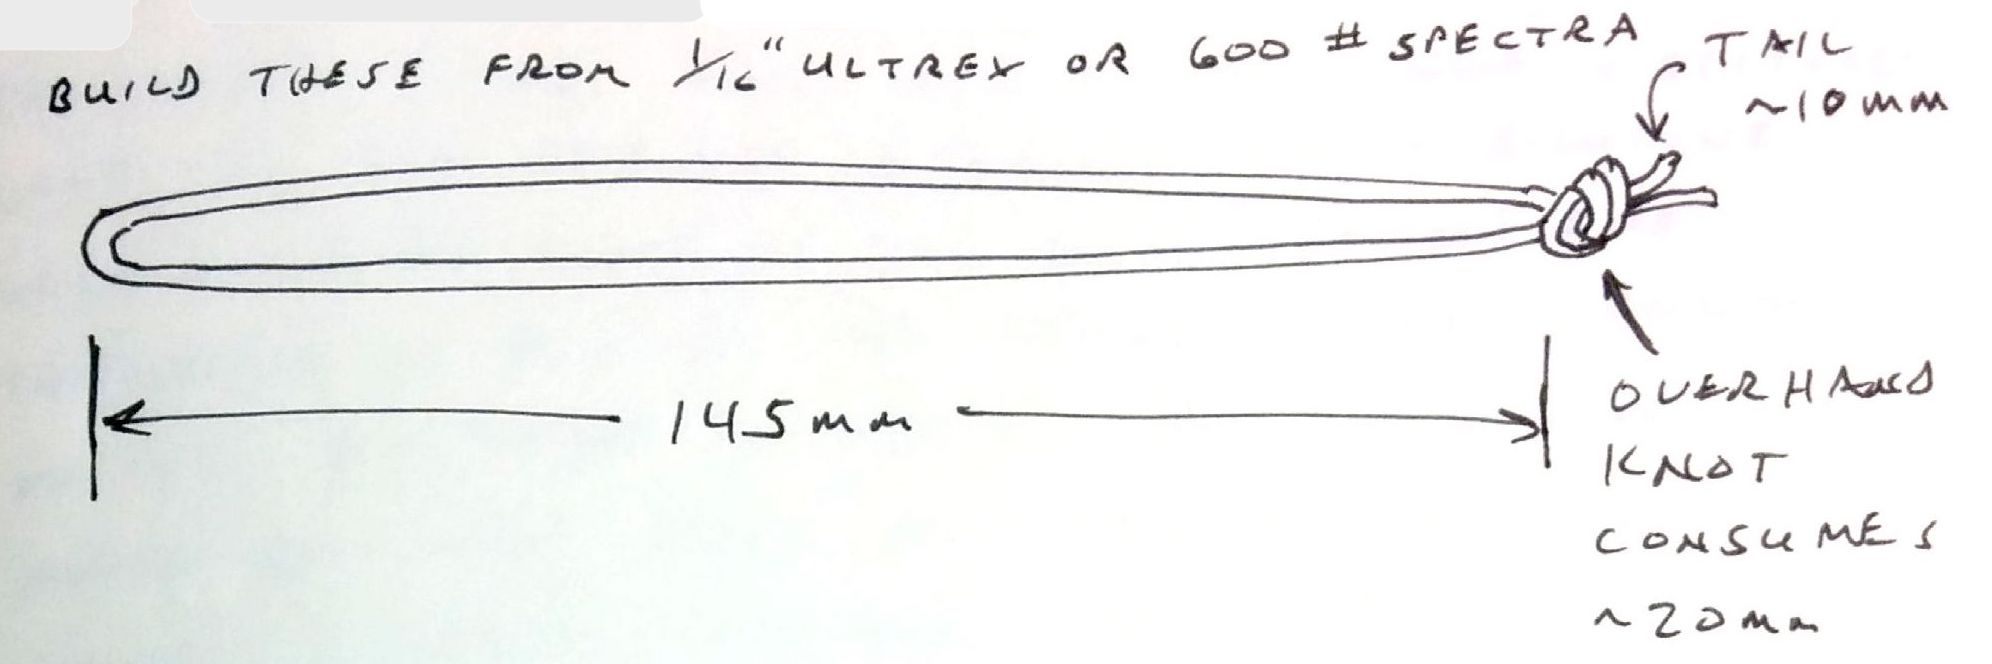
\includegraphics[width=0.7\linewidth]{images/05_kite_bar_rigging_2015-10-06_3} 

}

\caption{Bar End Loop}\label{fig:bar-end-loop}
\end{figure}

\hypertarget{steering-lines}{%
\section{Steering Lines}\label{steering-lines}}

The steering lines run from the bar end loops to the ends of the back lines. They require two 1140mm segments of 1/16" Ultrex 12. Mark each segment at 110, 190, 270, and 410mm. Use these marks to create a brummel splice with an 80mm loop.

With the loops complete, stretch the pair of lines evenly and mark both lines at about 25mm from the non-loop end. Tie and overhand knot in each line at the mark. Gently pinch the line with an adjustable wrench on the loop side of the knots. Use the wrench to pull the knots evenly while you pull the ends with standard pliers. With the knot complete and the lines equal in length, put little cyanoacrylate glue on the line ends to prevent fraying. See the construction details in Figure \ref{fig:steering-lines}.

\begin{figure}

{\centering 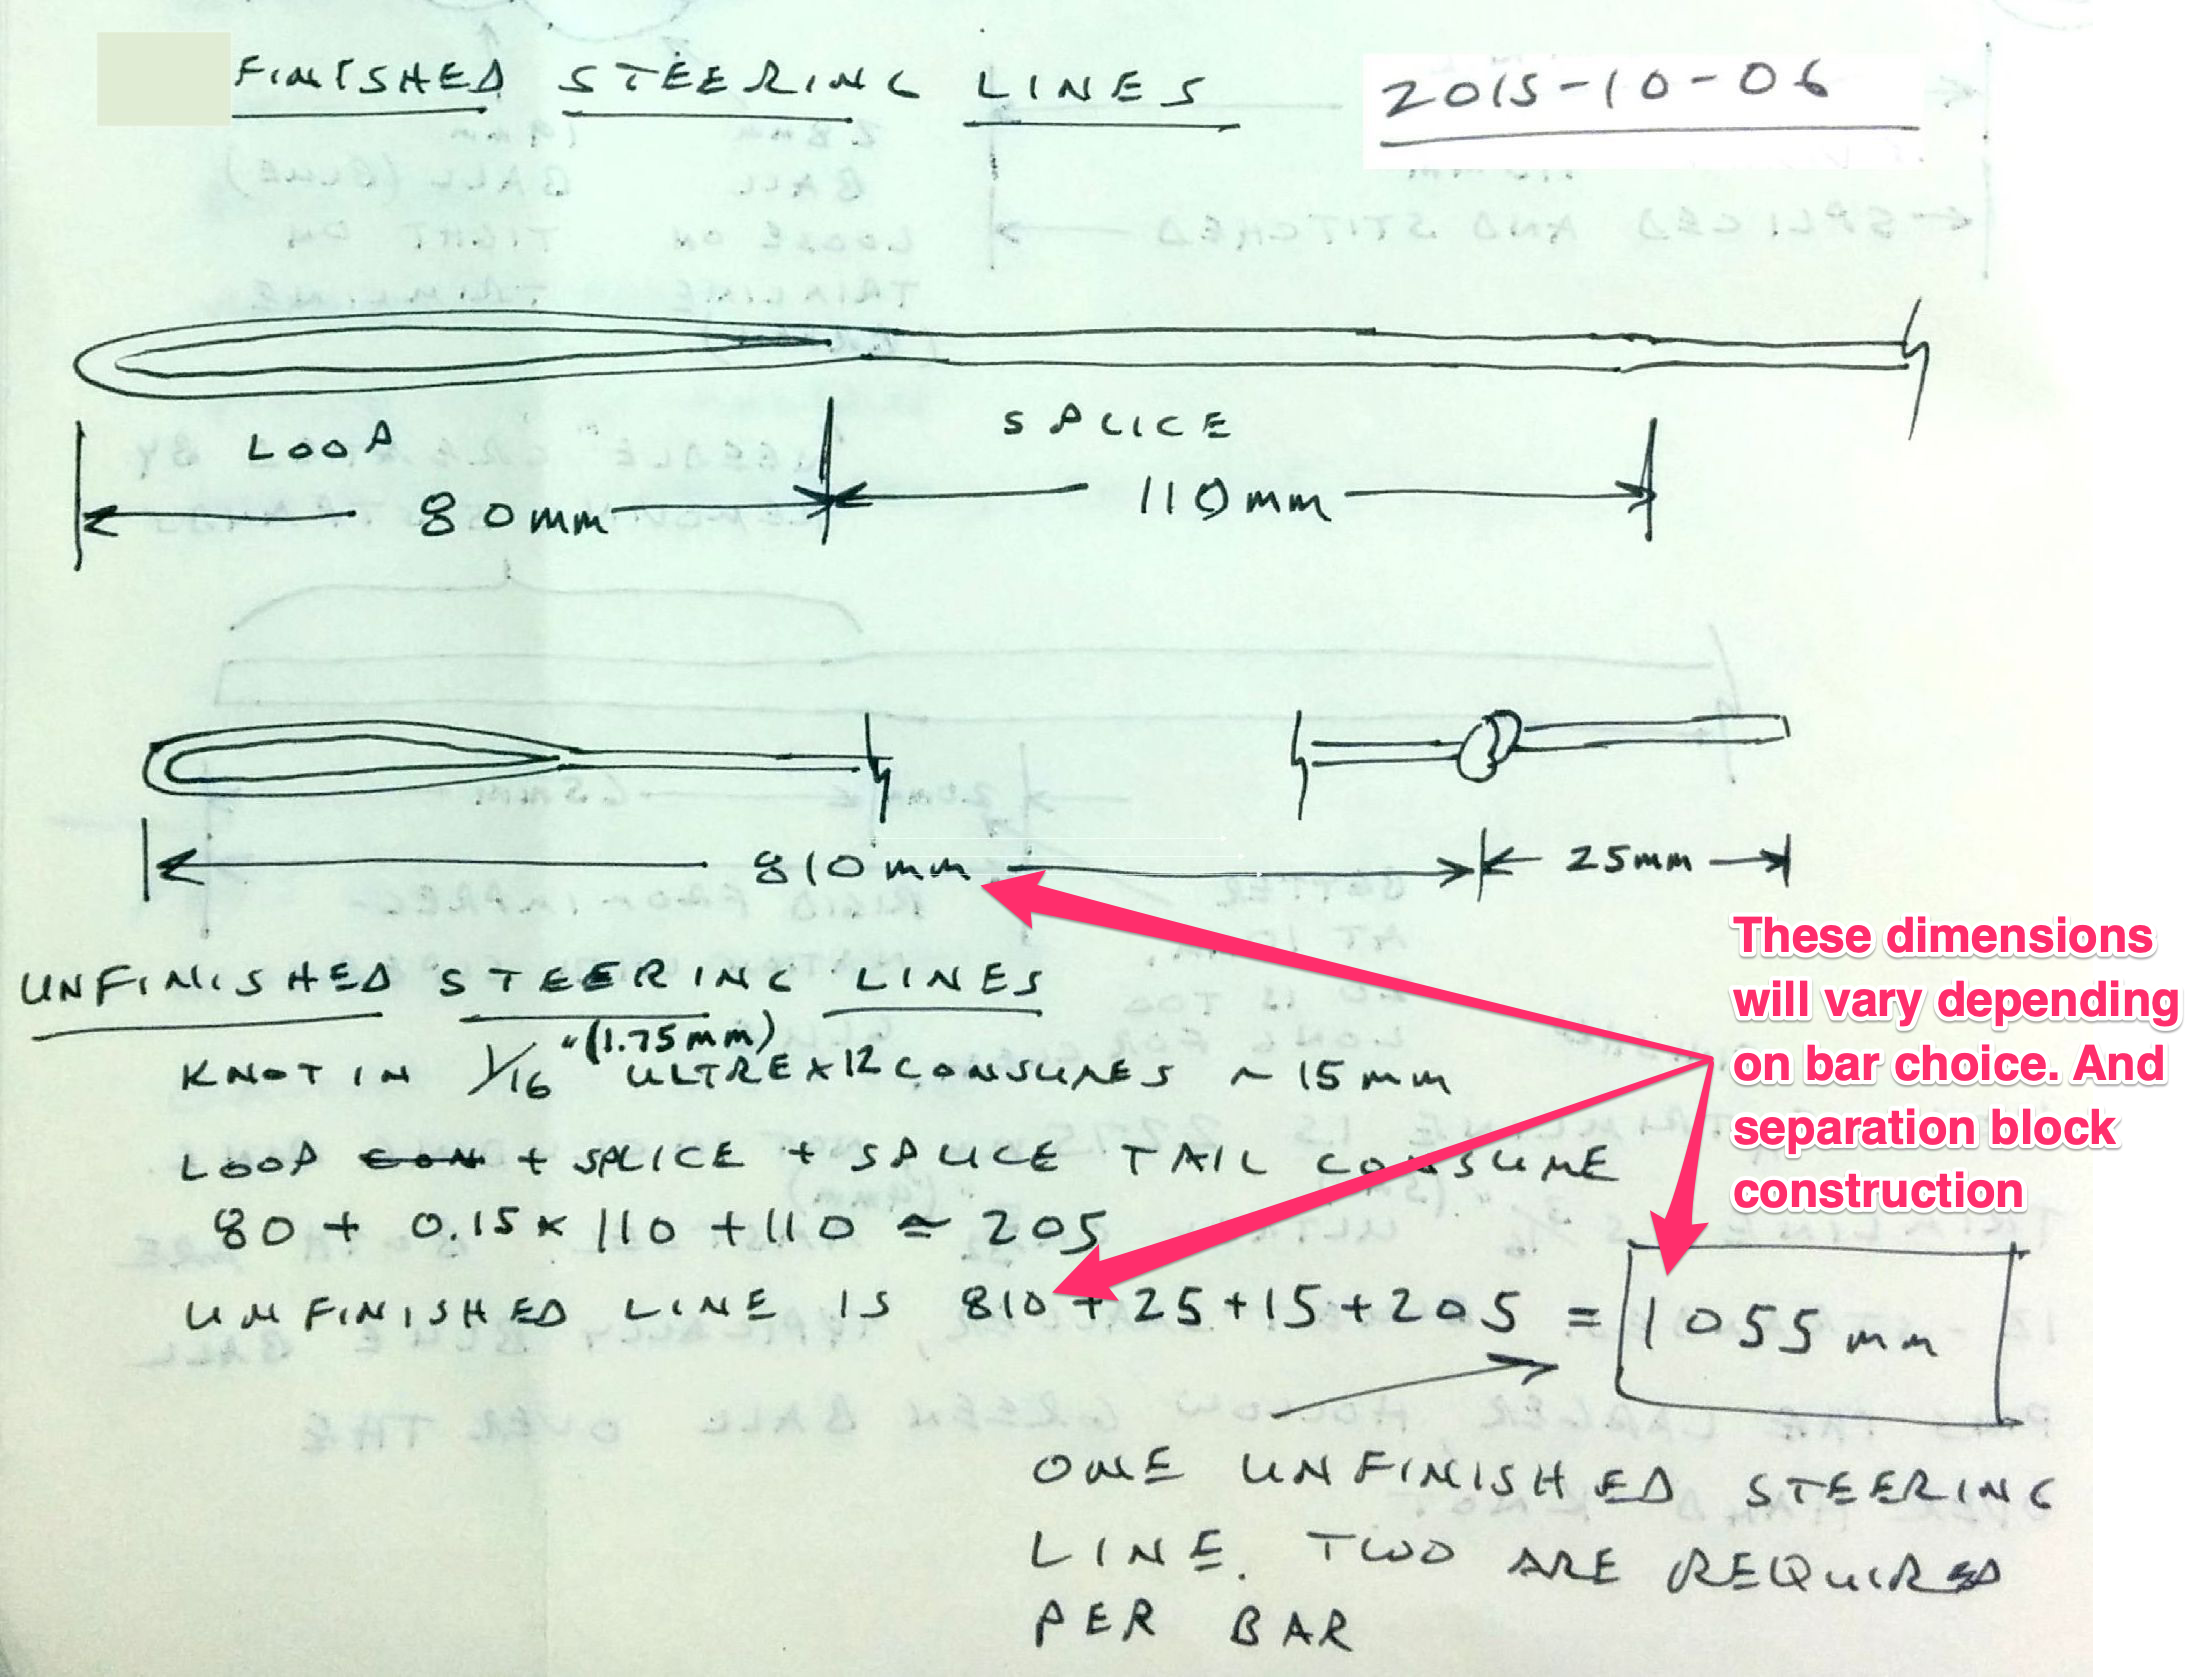
\includegraphics[width=0.7\linewidth]{images/04_kite_bar_rigging_2015-10-06_2} 

}

\caption{Steering line construction details}\label{fig:steering-lines}
\end{figure}

\hypertarget{assembly}{%
\chapter{Assembly}\label{assembly}}

\hypertarget{bar-assembly-and-threading-line}{%
\section{Bar assembly and threading line}\label{bar-assembly-and-threading-line}}

To thread the trim line, put the threaded end through the cleat, entering at the jam side. Exit the cleat at the top, routing up through the low friction ring of the separation block. Reenter the cleat and go through its serpentine path. Leave just enough line above the cleat to provide the desired trim. Route the line through the cleat bead. Go down through the center of the bar, through a \textasciitilde{}25mm ball to retain the trim line in the bar. Then go back through the center bore of the bar and through the cleat bead. Slide the cleat beaddown towards the bar to leave lots of slack next to the cleat. Before going any further, make sure the line already passing through the cleat's serpentine has 5 cm of loop on each side of the cleat. You'll need this slack in the next step.

Then route the loose end of the trim line \emph{up} through the cleat's serpentine path. You want to make large parallel loops of line going back and forth through the serpentine. Route about 5cm of the trim out of the top of the cleat.

\begin{figure}

{\centering 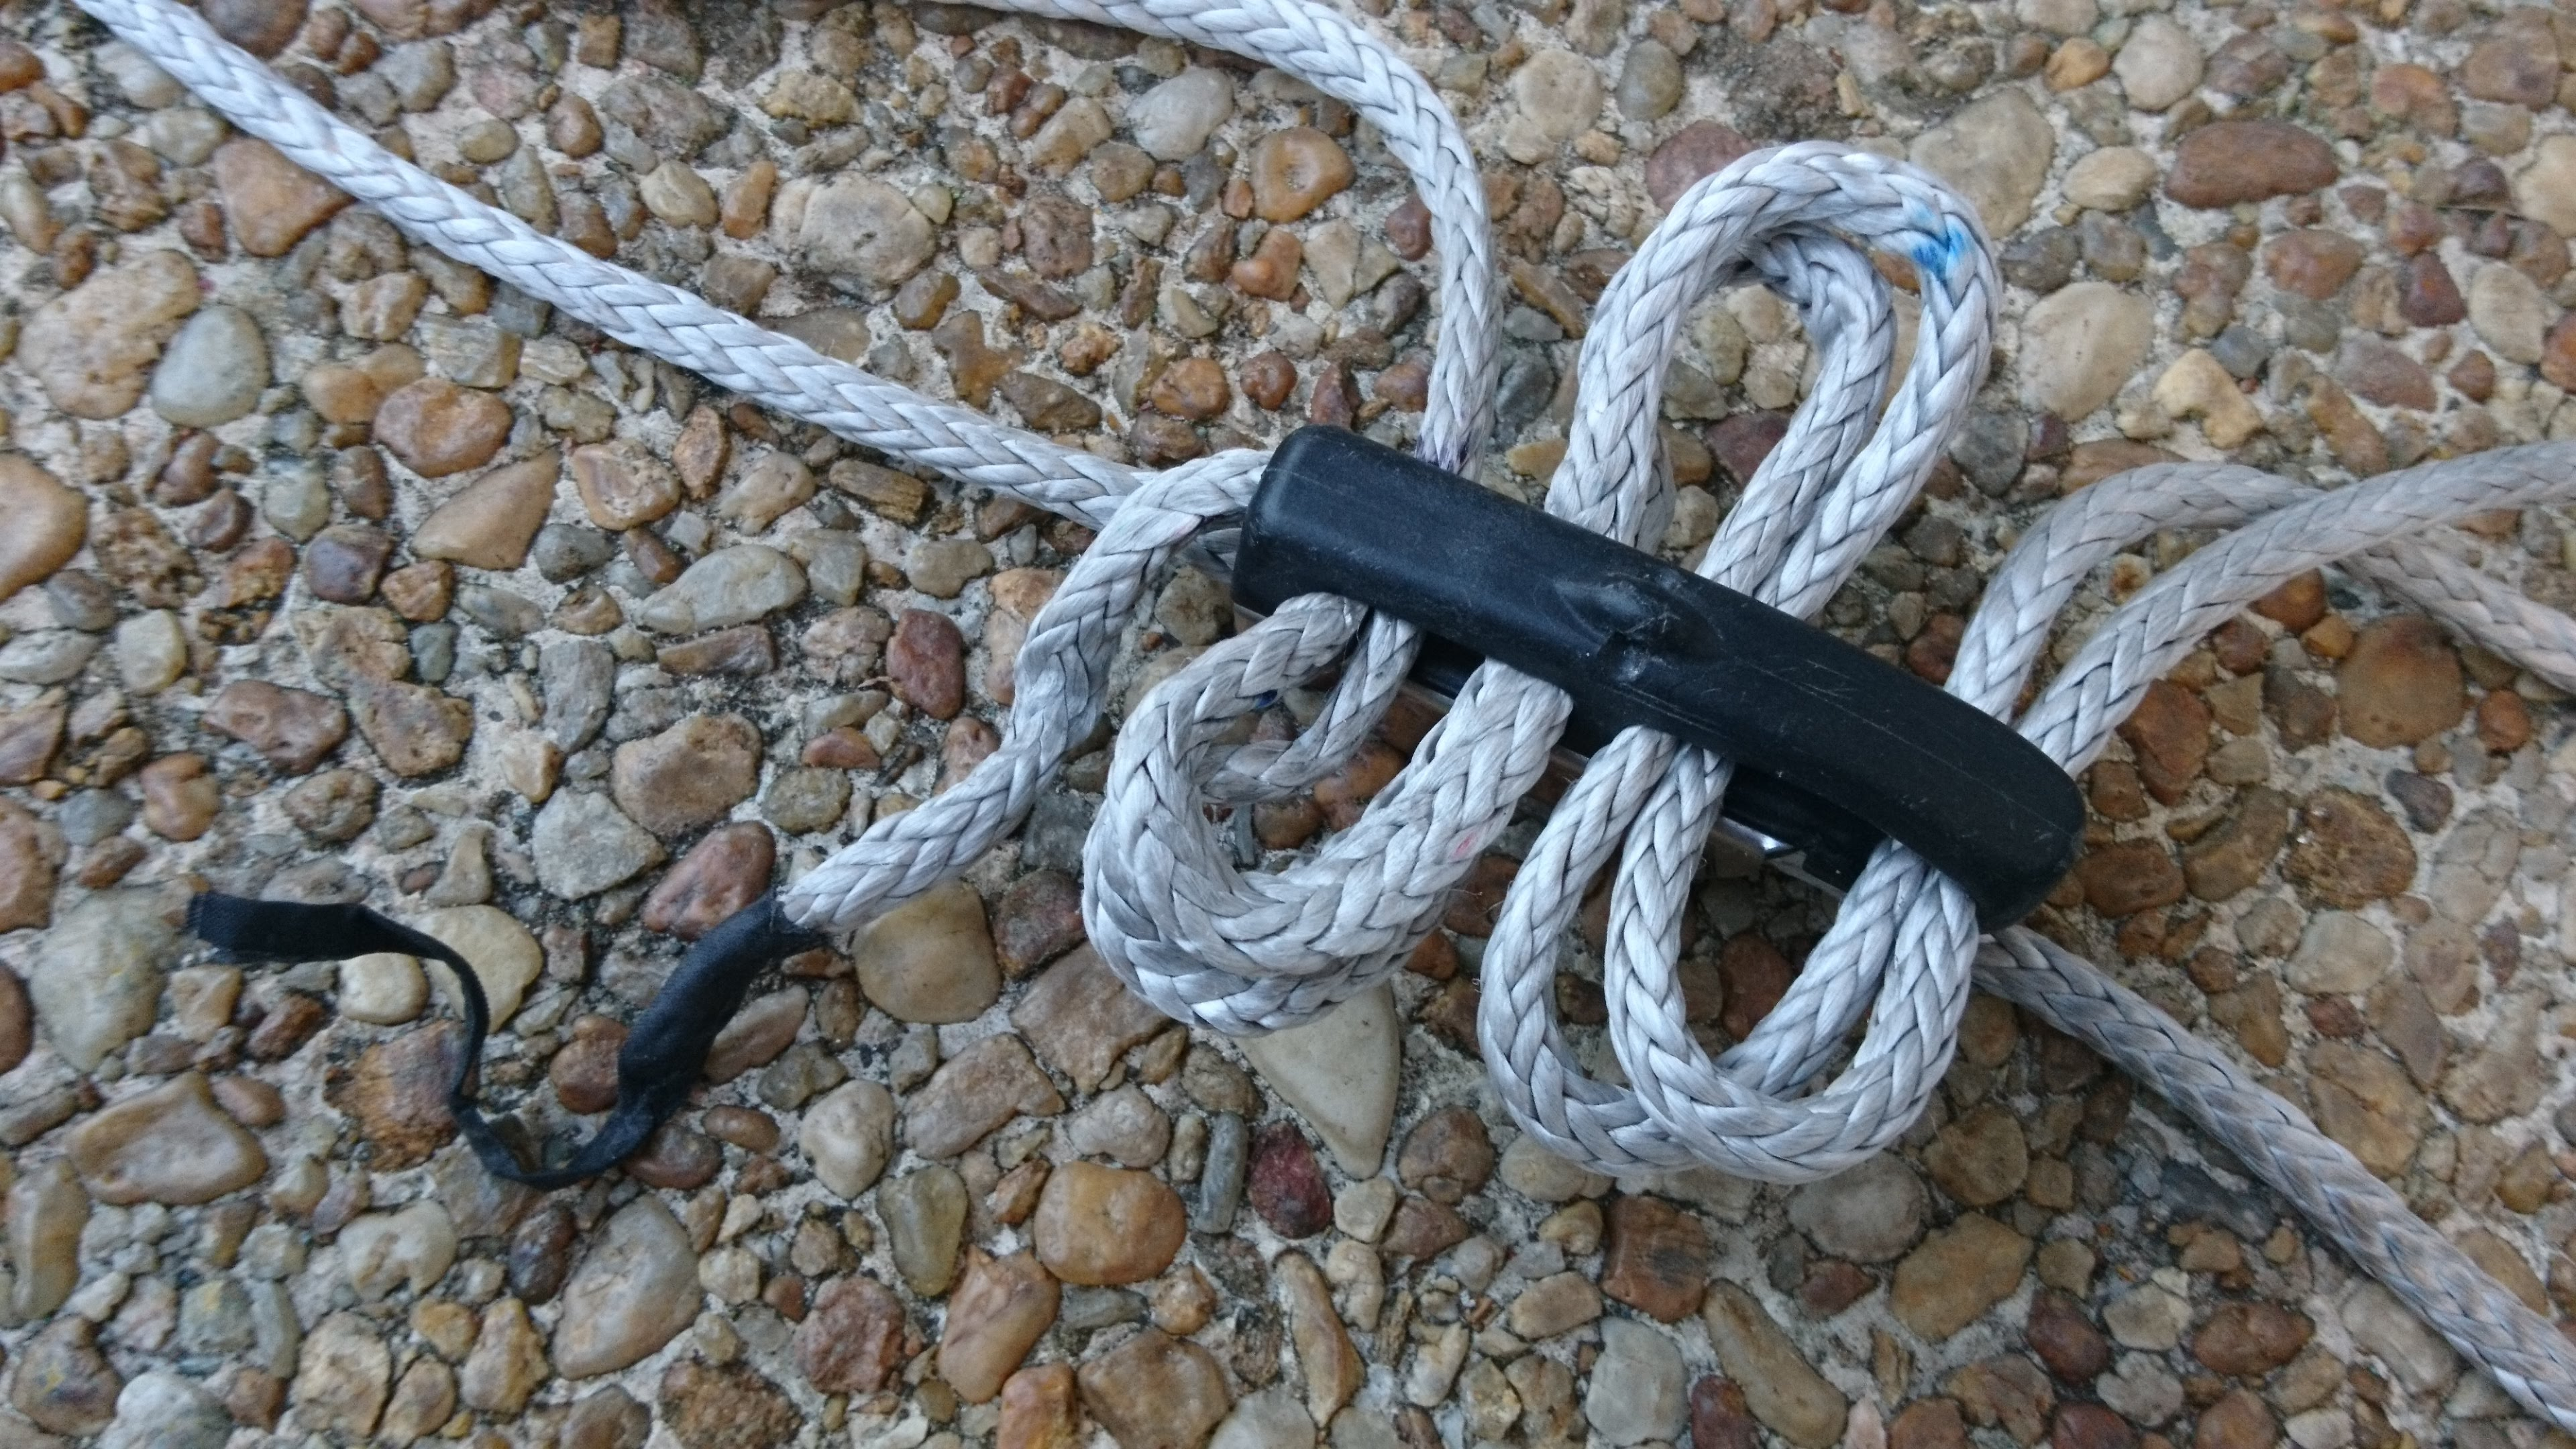
\includegraphics[width=0.7\linewidth]{images/threading_the_cleat_1} 

}

\caption{Form large parallel loops of line on each side of the cleat's serpentine path. Route about 5cm of the trim out of the top of the cleat.}\label{fig:thread-cleat-1}
\end{figure}

\begin{figure}

{\centering 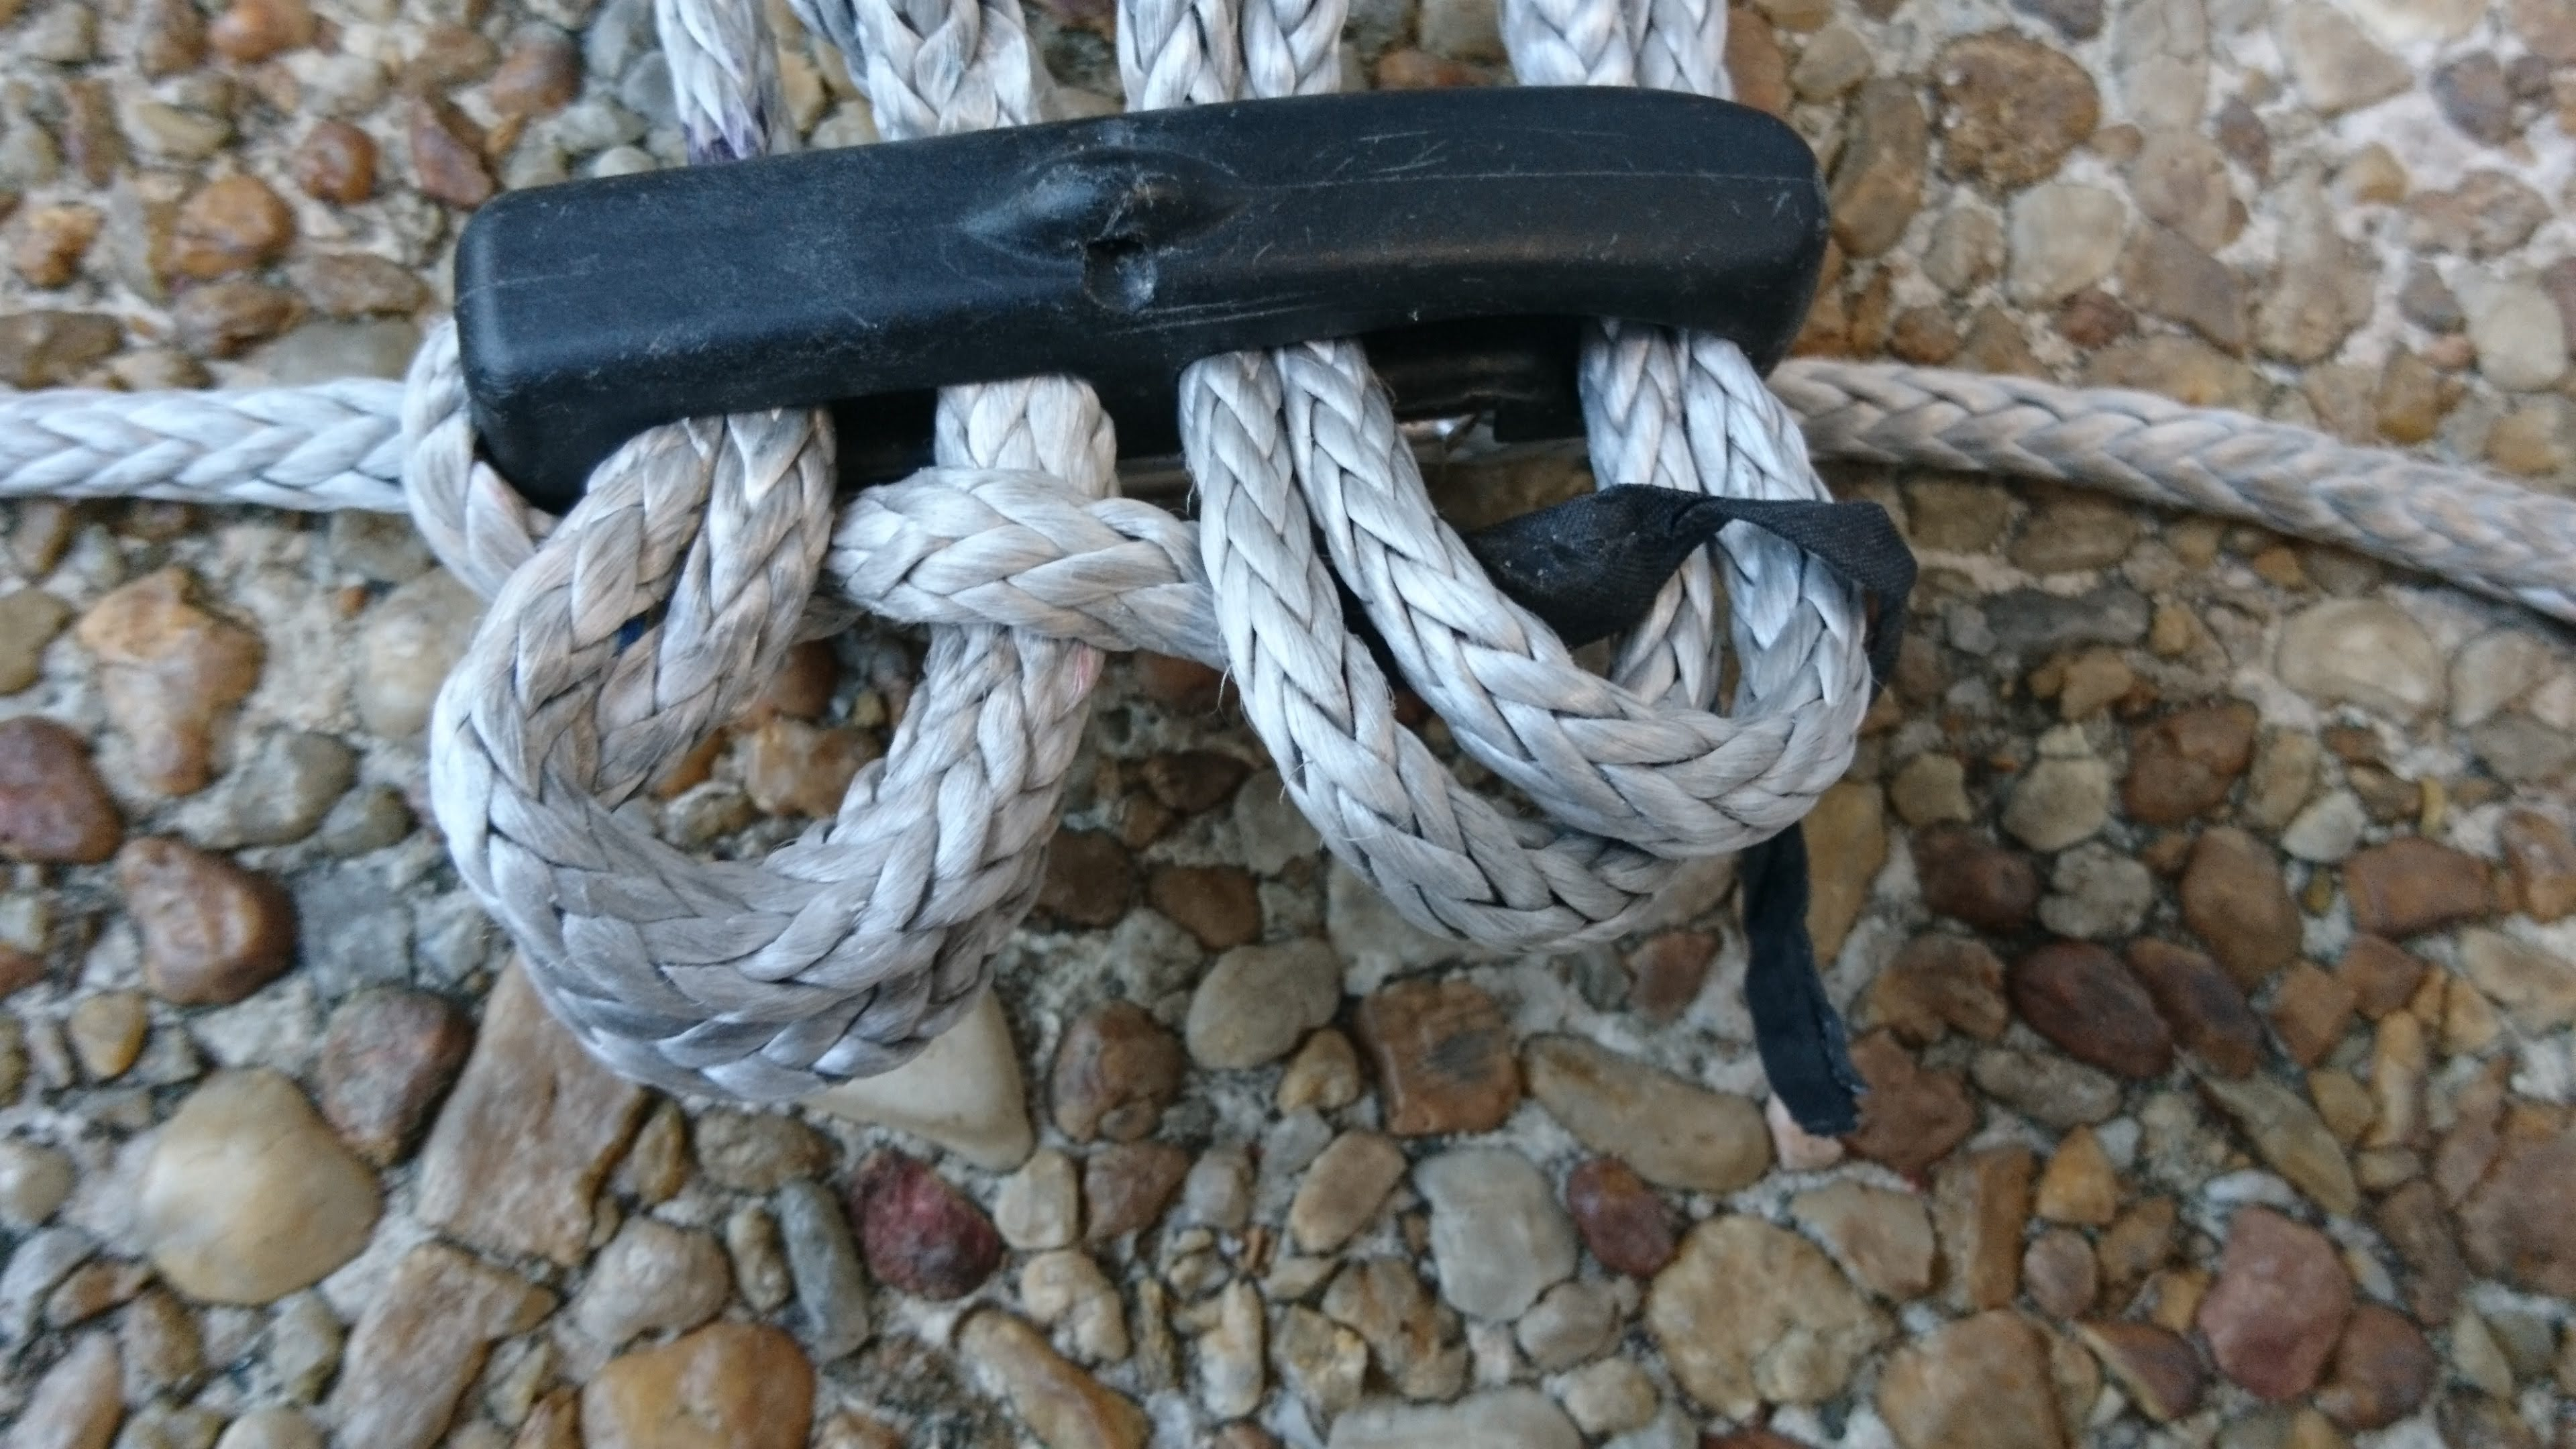
\includegraphics[width=0.7\linewidth]{images/threading_the_cleat_2} 

}

\caption{Route the 5cm of trim line tail through the loops along the side of the serpentine.}\label{fig:thread-cleat-2}
\end{figure}

\begin{figure}

{\centering 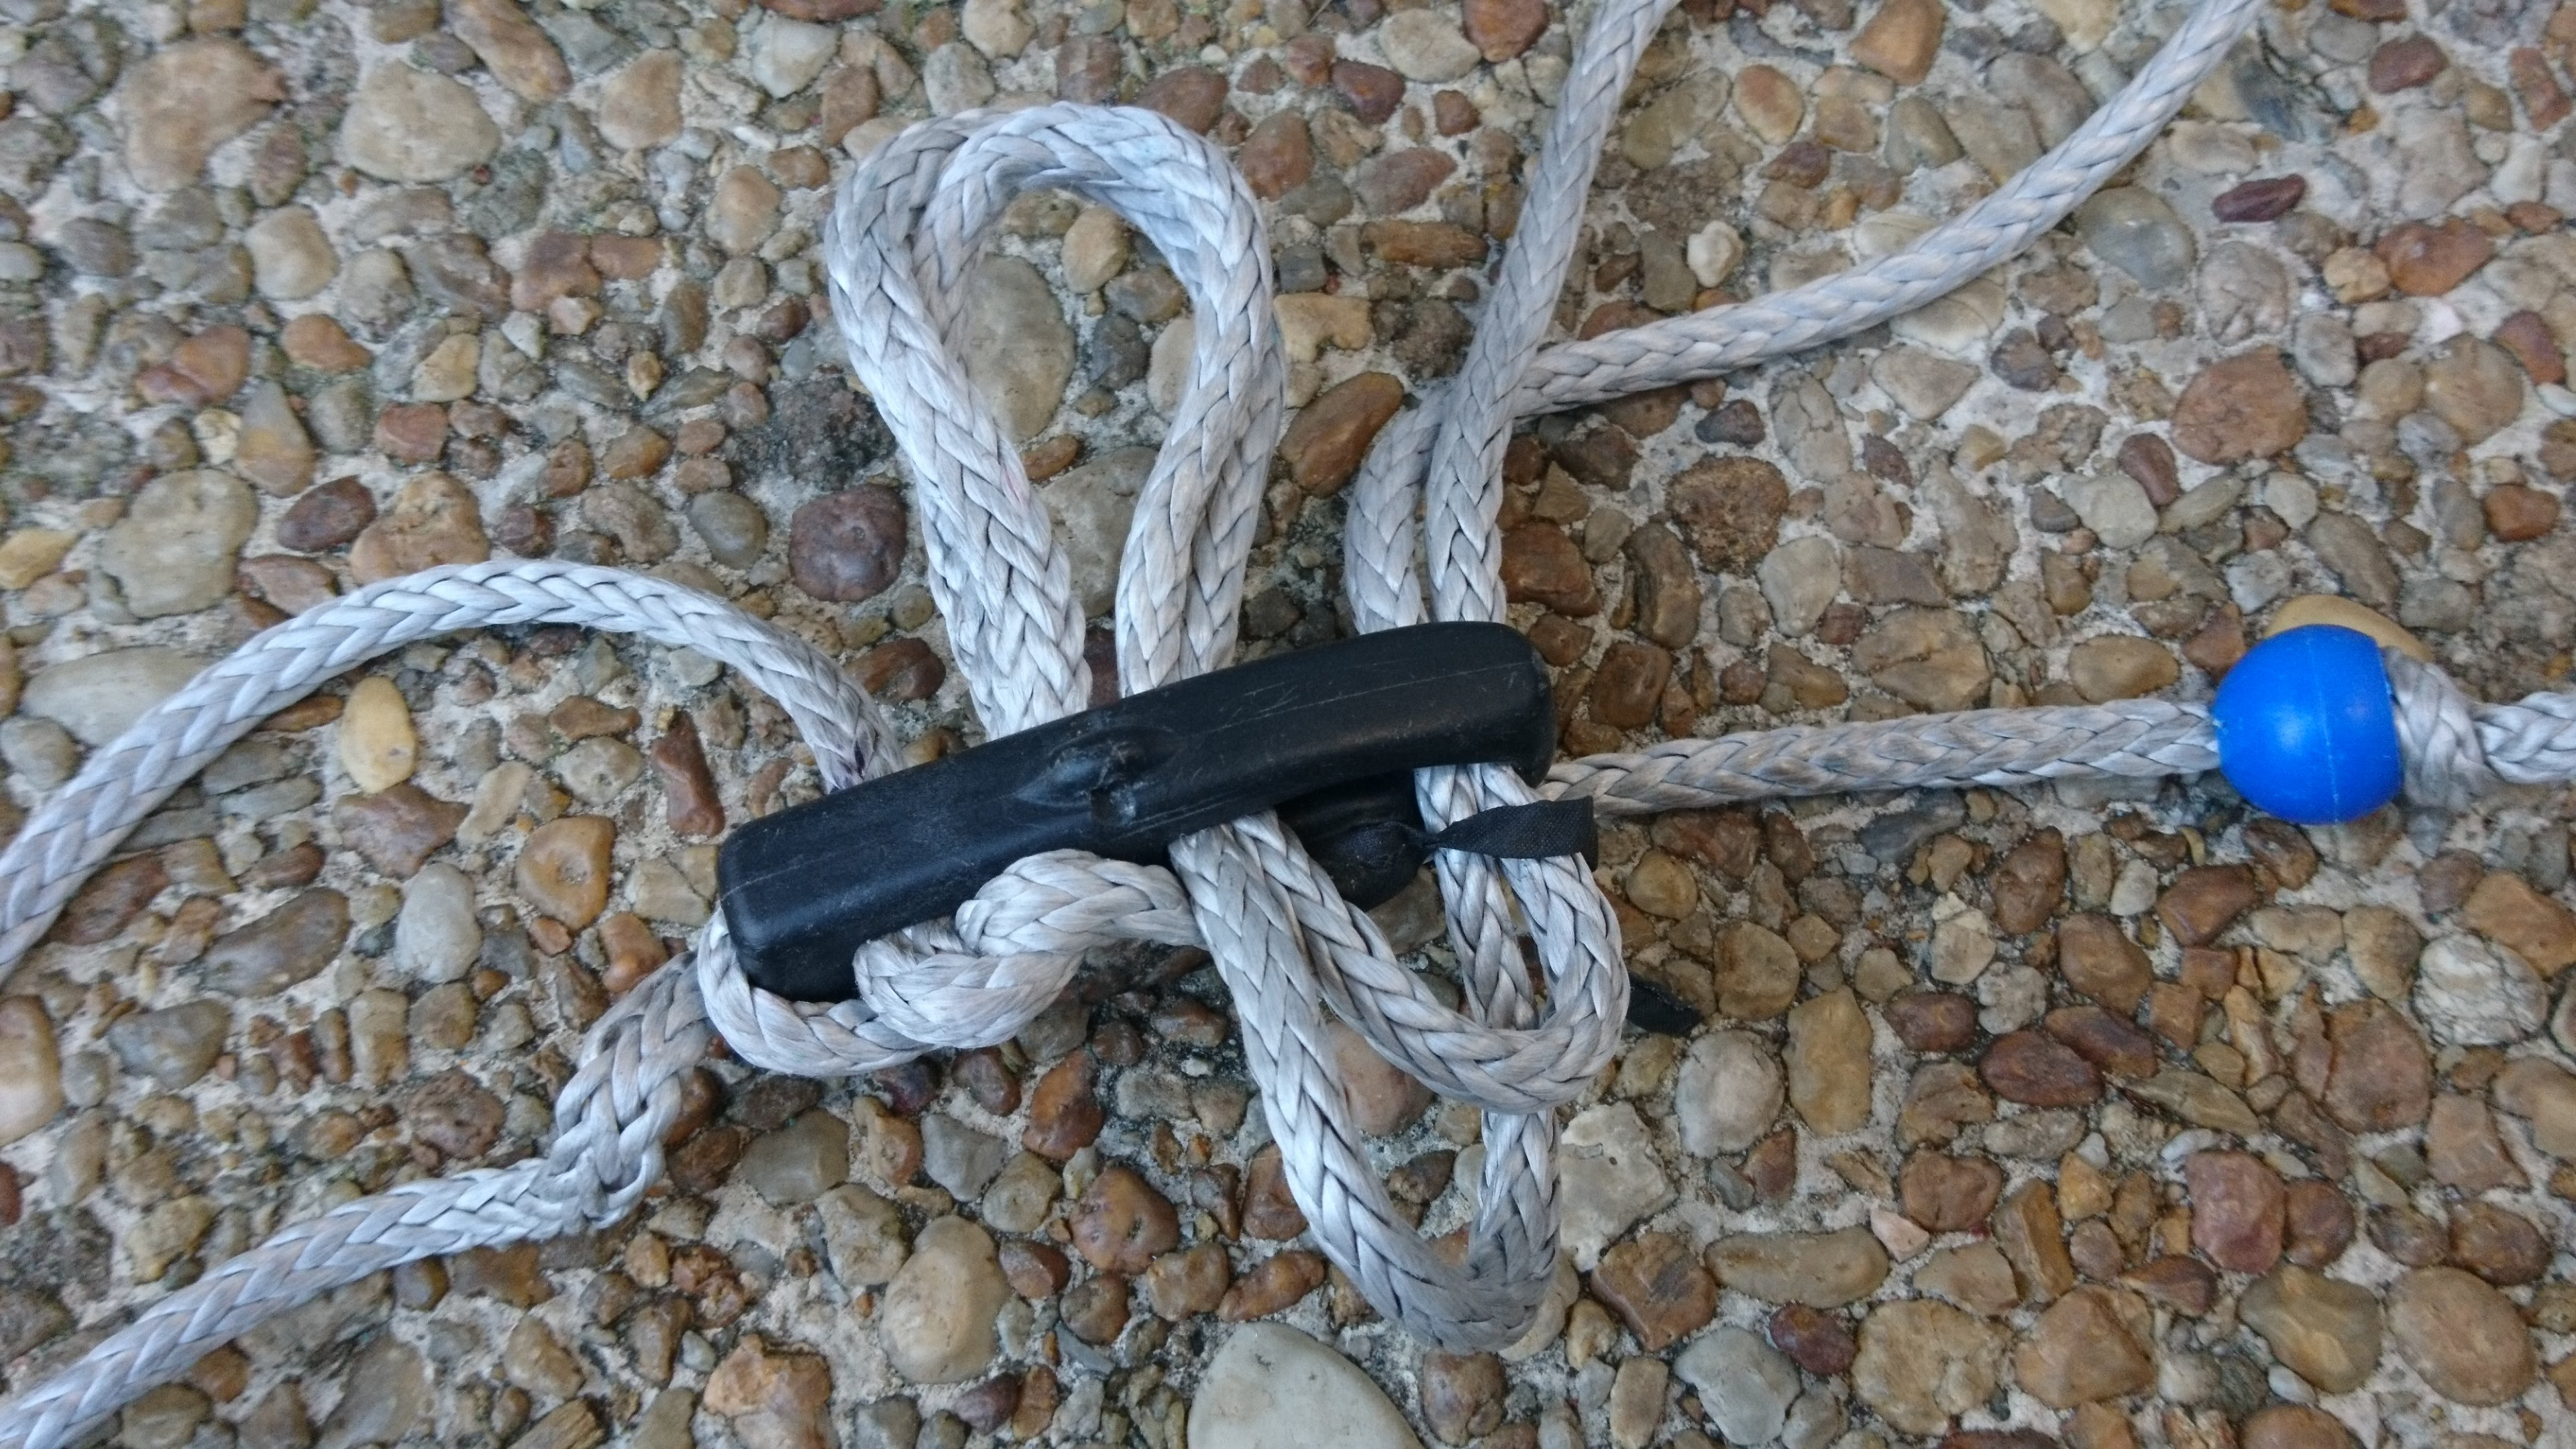
\includegraphics[width=0.7\linewidth]{images/threading_the_cleat_3} 

}

\caption{Route the insignia cloth tail through the loops. Holding the tail in place, pull the trim line slack down through the cleat grooming the lines as you go. Keep the lines as parallel as possible. Take the slack out of the trimline loops 1 of 3.}\label{fig:thread-cleat-3}
\end{figure}

\begin{figure}

{\centering 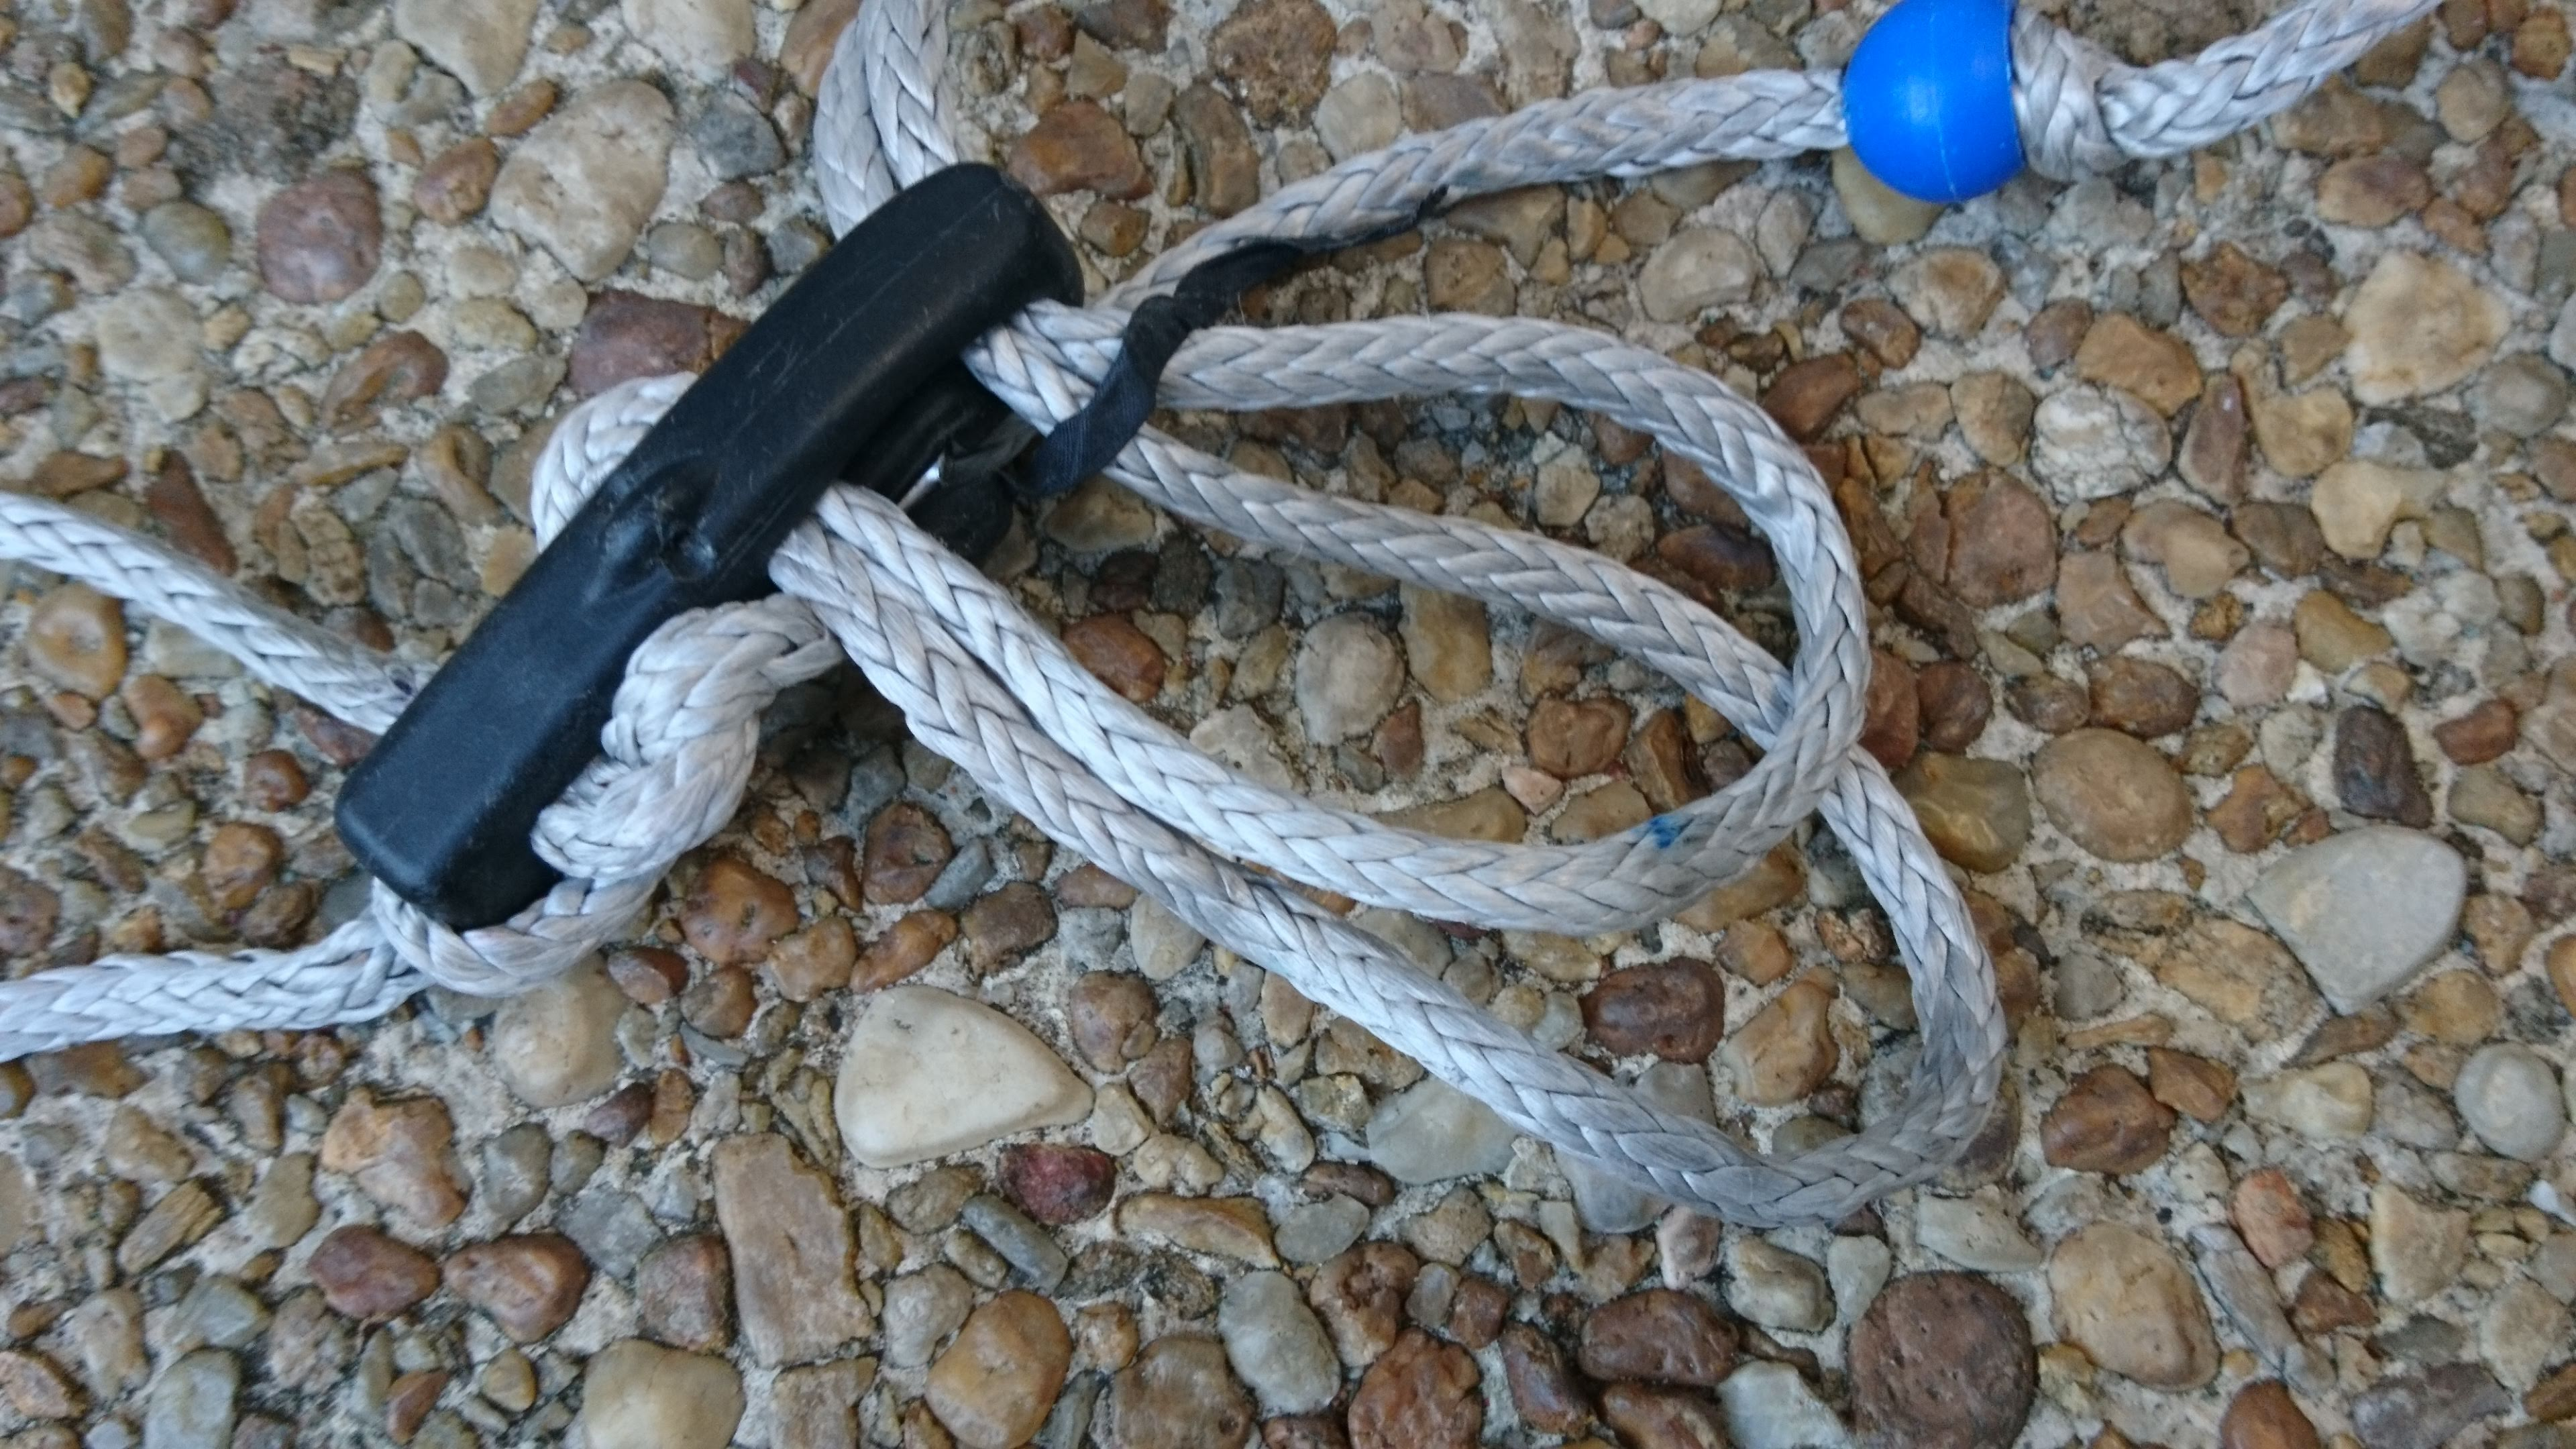
\includegraphics[width=0.7\linewidth]{images/threading_the_cleat_4} 

}

\caption{Take the slack out of the trimline loops 2 of 3.}\label{fig:thread-cleat-4}
\end{figure}

\begin{figure}

{\centering 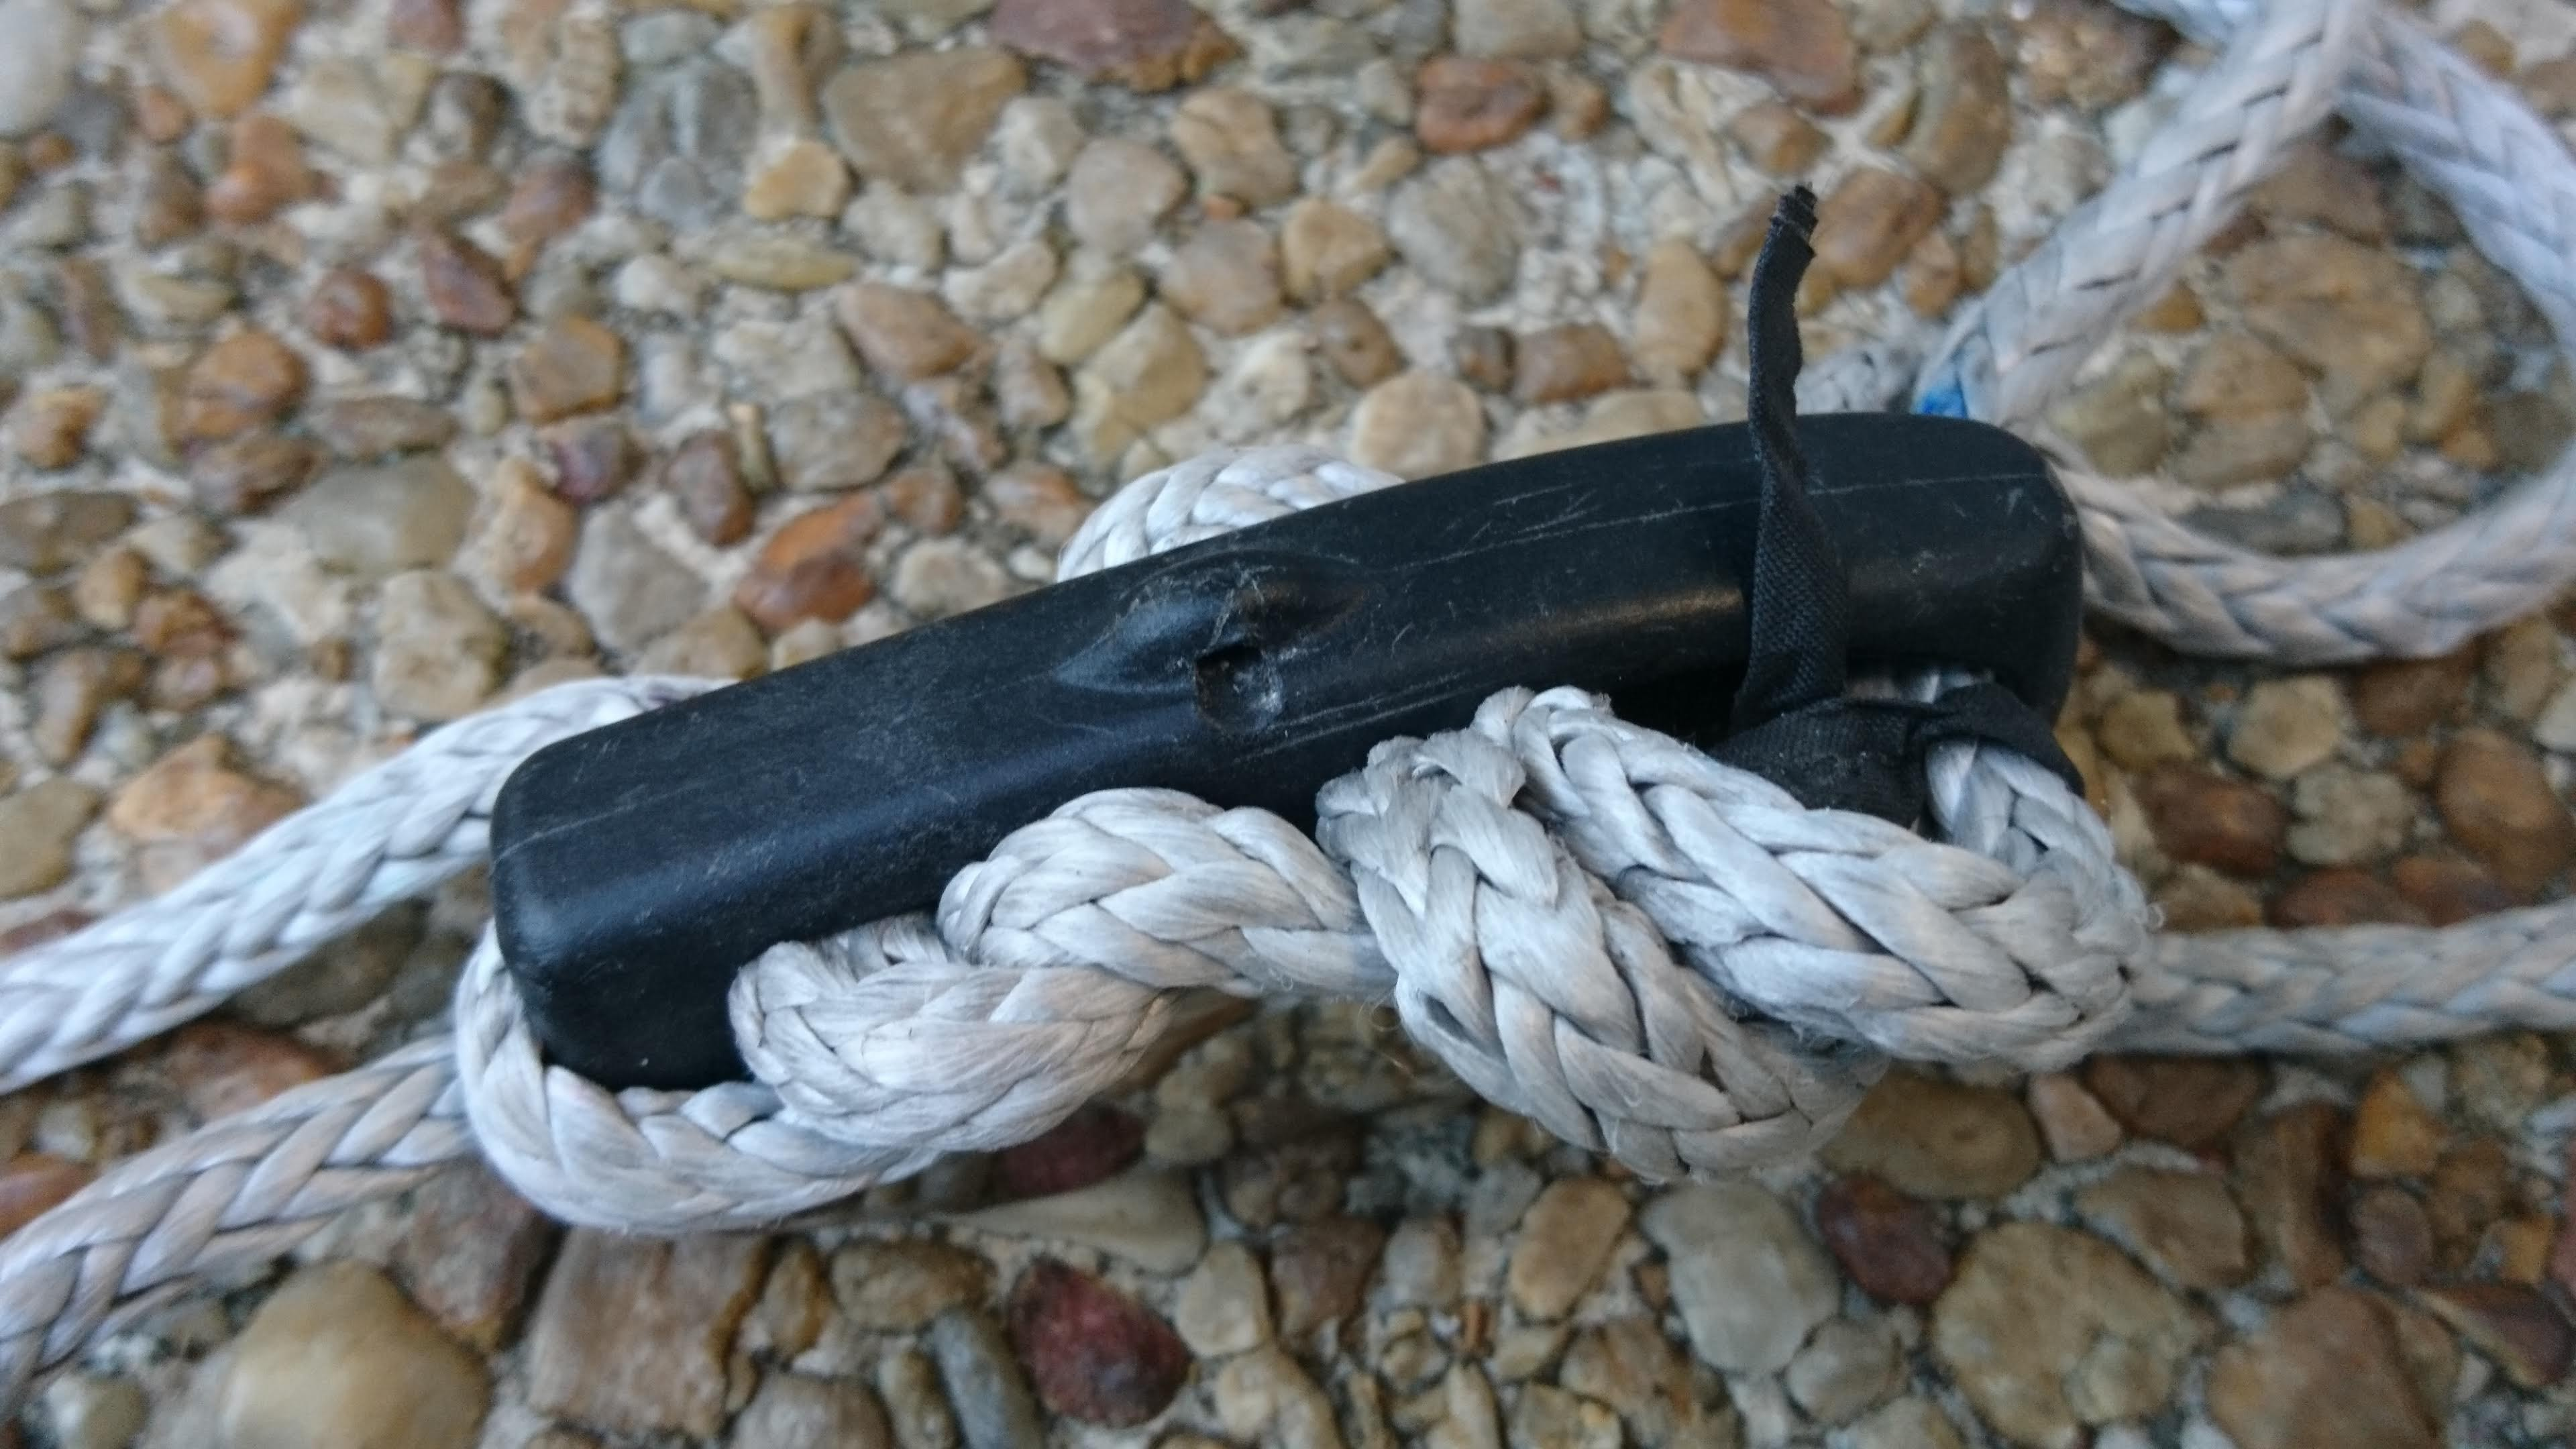
\includegraphics[width=0.7\linewidth]{images/threading_the_cleat_5} 

}

\caption{Take the slack out of the trimline loops 3 of 3.}\label{fig:thread-cleat-5}
\end{figure}

With the trimline tight in the serpentine path, have a friend help you put the trim line in tension. Then slide the cleat bead up to the cleat. Look at the cleat from the pilot's point of view and rotatecleat until the jaws are up. Check the rotation of the cleat bead so that the flag line guide path is on the lower left side of the cleat. Pull the trim lines and jam the bead onto the bottom of the cleat.

You'll want to verify you can reach the trimline end under normal flying conditions. It's easier to assess the cleat position before the flying lines are attached so pause the assembly for a moment to check and adjust the cleat position. To do this, put your harness on, clip the trim line into the harness and have a friend pull on the trim line by the separation block. They should pull the bar to your side about 30 degrees above horizontal. Verify you can reach the jaws of the cleat and grab the trim line tail without over-reaching. If you have to stretch to reach the tail, the cleat is too far away. You can move it closer by moving some of the trim line up through the cleat. For each centimeter you need to move the cleat down, you'll need to move two centimeters of line through the cleat. Making this adjustment is a bit tedious, but the trim line tail must be in easy reach under load.

\hypertarget{attaching-the-flying-lines}{%
\section{Attaching the flying lines}\label{attaching-the-flying-lines}}

With the trim line routed, the flying lines can be attached. Route one the flying lines down through the separation block and attach the stub line stopper to the end-loop of the flying line with a larks head to retain the flying line in the stopper.

Route the other flying line through the remaining hole in the separation block. Continue routing it through the cleat bead and then the bar. Attach the flag line to the flying line with a larks head. Pull flag line up through the bar and bead with the flying line. The routed lines should look like Figure \ref{fig:flag-line-at-separation-block} at the separation block. The over-all assembly should look like \ref{fig:upper-section-of-assembled-bar}

\begin{figure}

{\centering 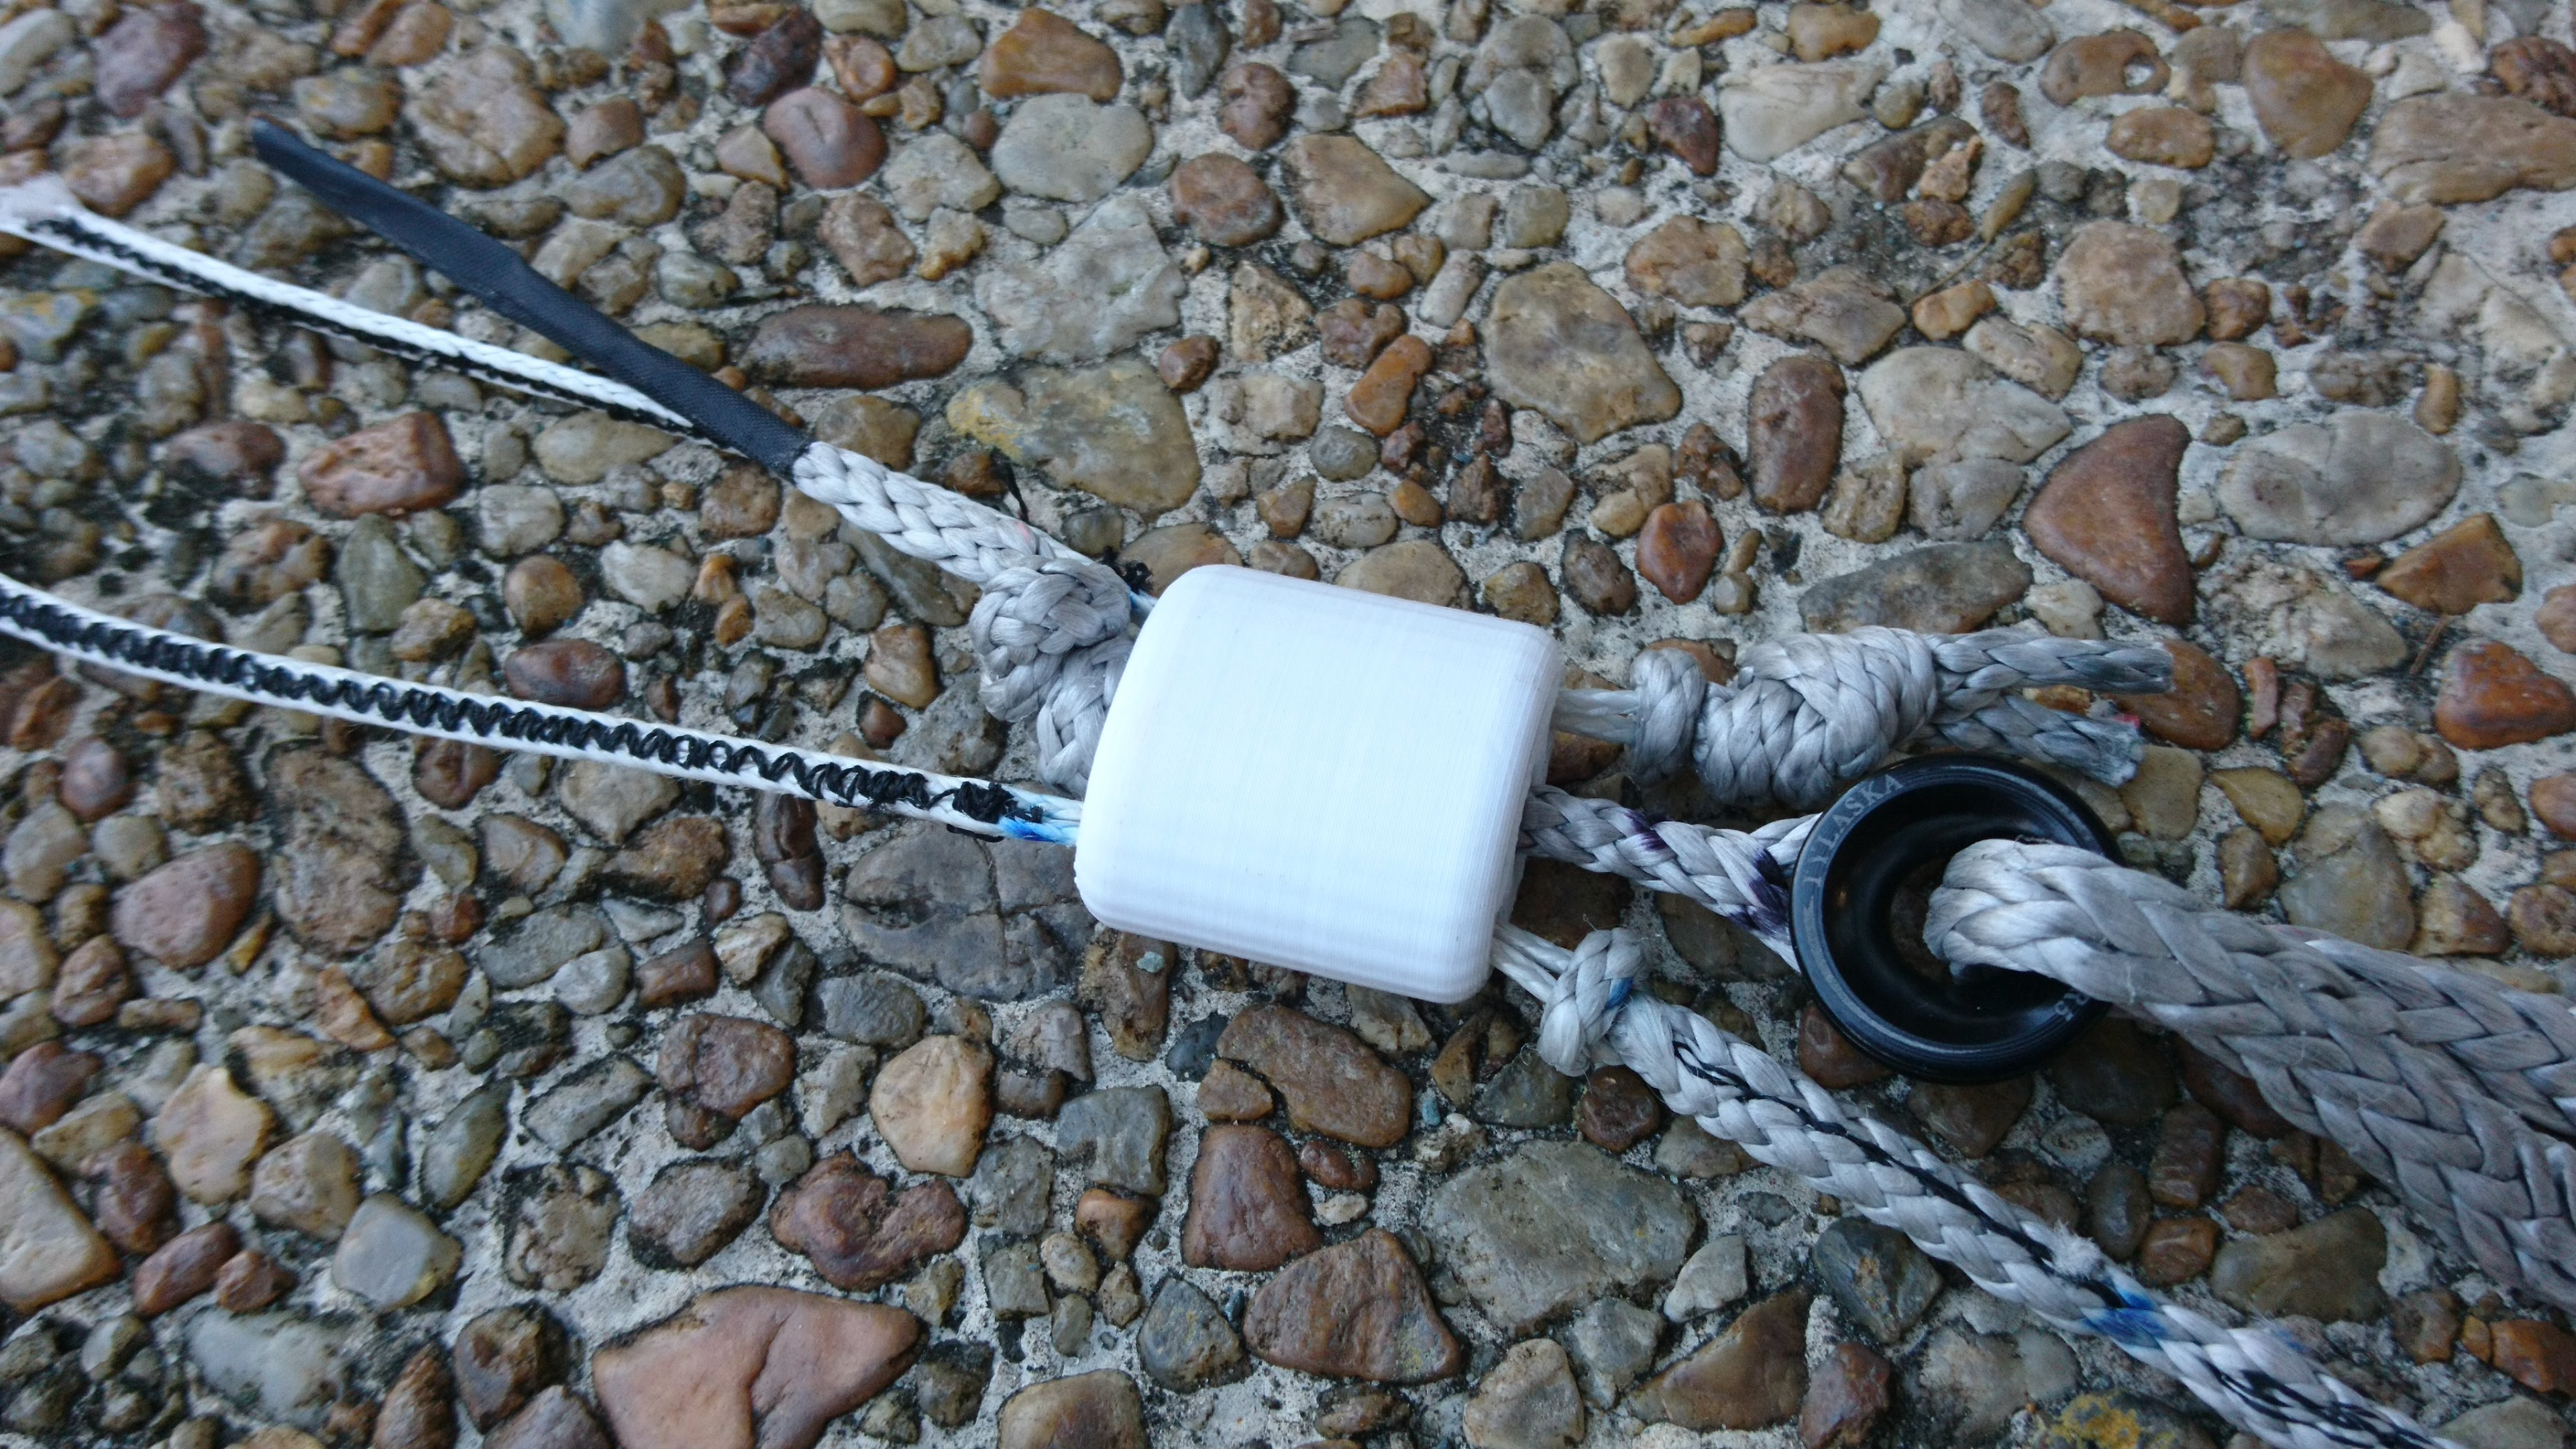
\includegraphics[width=0.7\linewidth]{images/flag-line-at-separation-block} 

}

\caption{The flag line meets the flying line.}\label{fig:flag-line-at-separation-block}
\end{figure}

\begin{figure}

{\centering 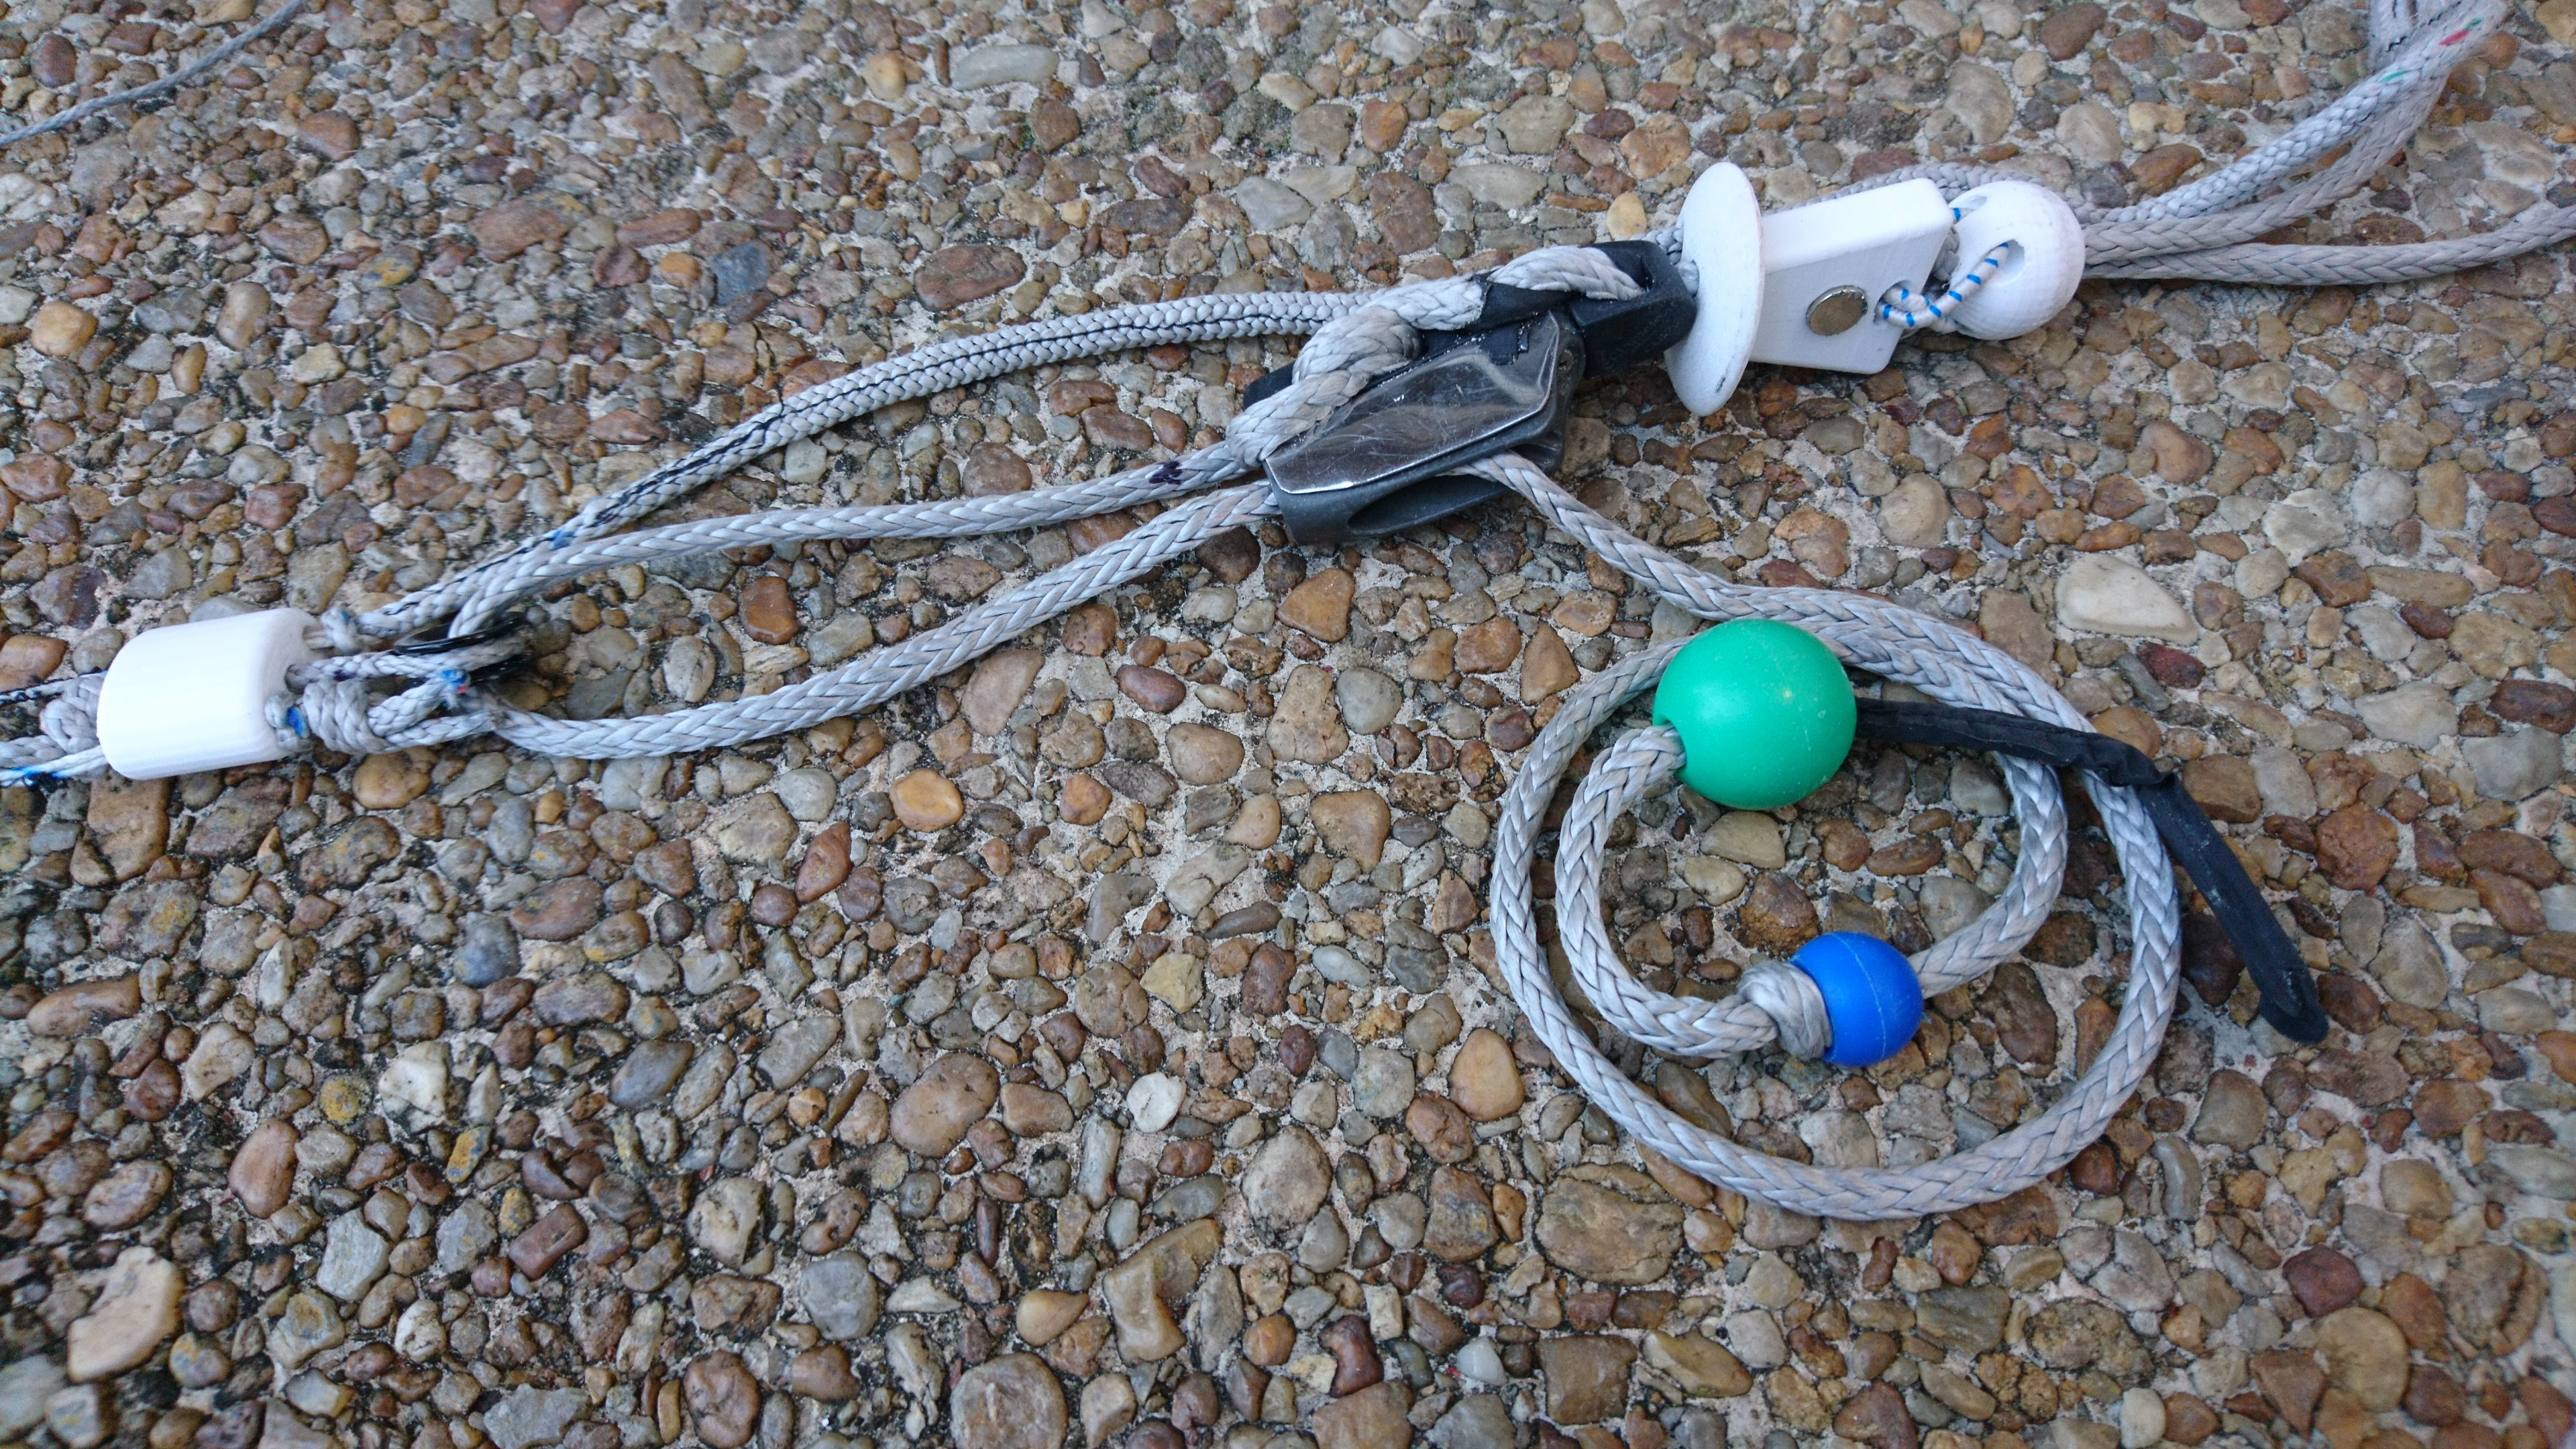
\includegraphics[width=0.7\linewidth]{images/upper_section_of_assembled_bar} 

}

\caption{Assembled bar}\label{fig:upper-section-of-assembled-bar}
\end{figure}

\hypertarget{bar-end-loops-1}{%
\section{Bar End Loops}\label{bar-end-loops-1}}

Pull each bar end loop through one of the holes at the ends of the bar. Route the loop from the pilot-side of the bar to the kite side so the knots are left on the pilot side. Make sure both sides of the loop are even and the knot sits flush against the back of the bar.

\hypertarget{steering-line-leaders}{%
\section{Steering line leaders}\label{steering-line-leaders}}

Use a larkshead to attach the loop of each steering line leader to the loop of its steering line. Then attach the knot of the leader to the loop of the bar-end loop with a larks head. Keeping the knot of the leaderline next to the bar minimizes the risk of snagging the steering lines in the components of the bar.

With all the lines attached, the trim control let all the way out and the bar pulled all the way back, the tips of all four flying lines should converge to the same point.

\bibliography{book.bib,packages.bib}


\end{document}
